% CREATED BY WOLFGANG AHRENDT, 2021
% BASED ON A MASTER THESIS TEMPLATE CREATED BY DAVID FRISK, 2016,
%        MODIFIED BY JAKOB JARMAR 2016 AND GUSTAV ÖRTENBERG 2019

% IMPORT SETTINGS
\documentclass[12pt,a4paper]{report}
% CREATED BY DAVID FRISK, 2016
\usepackage{listings}
\usepackage{xcolor}
\usepackage{svg}
\definecolor{codegreen}{rgb}{0,0.6,0}
\definecolor{codegray}{rgb}{0.5,0.5,0.5}
\definecolor{codepurple}{rgb}{0.58,0,0.82}
\definecolor{backcolour}{rgb}{0.95,0.95,0.92}
\lstdefinestyle{mystyle}{
    backgroundcolor=\color{backcolour},   
    commentstyle=\color{codegreen},
    keywordstyle=\color{magenta},
    numberstyle=\tiny\color{codegray},
    stringstyle=\color{codepurple},
    basicstyle=\ttfamily\footnotesize,
    breakatwhitespace=false,         
    breaklines=true,                 
    captionpos=b,                    
    keepspaces=true,                 
    numbers=left,                    
    numbersep=5pt,                  
    showspaces=false,                
    showstringspaces=false,
    showtabs=false,                  
    tabsize=2
}
\lstset{style=mystyle}

% BASIC SETTINGS

\usepackage{moreverb}								% List settings
\usepackage{textcomp}								% Fonts, symbols etc.
\usepackage{lmodern}								% Latin modern font
\usepackage{helvet}									% Enables font switching
\usepackage[T1]{fontenc}							% Output settings
\usepackage[english]{babel}							% Language settings
\usepackage[utf8]{inputenc}							% Input settings
\usepackage{amsmath}								% Mathematical expressions (American mathematical society)
\usepackage{amssymb}								% Mathematical symbols (American mathematical society)
\usepackage{graphicx}								% Figures
\usepackage{caption}
\usepackage{subcaption}
%\usepackage{subfig}									% Enables subfigures
\numberwithin{equation}{chapter}					% Numbering order for equations
\numberwithin{figure}{chapter}						% Numbering order for figures
\numberwithin{table}{chapter}						% Numbering order for tables
%%try to recomment this isak
%\usepackage{minted}						    		% Enables source code listings
\usepackage{chemfig}								% Chemical structures
\usepackage[top=3cm, bottom=3cm,
			inner=3cm, outer=3cm]{geometry}			% Page margin lengths			
\usepackage{eso-pic}								% Create cover page background
\newcommand{\backgroundpic}[3]{
	\put(#1,#2){
	\parbox[b][\paperheight]{\paperwidth}{
	\centering
	\includegraphics[width=\paperwidth,height=\paperheight,keepaspectratio]{#3}}}}
\usepackage{float} 									% Enables object position enforcement using [H]
\usepackage{parskip}								% Enables vertical spaces correctly 
\usepackage{datetime} %date formatting tools


% OPTIONAL SETTINGS (DELETE OR COMMENT TO SUPRESS)

% Disable automatic indentation (equal to using \noindent)
\setlength{\parindent}{0cm}                         
\usepackage{csquotes}
% \begin{comment}
%      commented code
% \end{comment}
\usepackage{comment}

\usepackage{fancyvrb}

% Caption settings (aligned left with bold name)
\usepackage[labelfont=bf, textfont=normal,
			justification=justified,
			singlelinecheck=false]{caption} 		

		  	
% Activate clickable links in table of contents  	
\usepackage{hyperref}								
\hypersetup{colorlinks, citecolor=black,
   		 	filecolor=black, linkcolor=black,
    		urlcolor=black}


% Define the number of section levels to be included in the t.o.c. and numbered	(3 is default)	
\setcounter{tocdepth}{5}							
\setcounter{secnumdepth}{5}	


% Chapter title settings
\usepackage{titlesec}		
\titleformat{\chapter}[display]
  {\Huge\bfseries\filcenter}
  {{\fontsize{50pt}{1em}\vspace{-4.2ex}\selectfont \textnormal{\thechapter}}}{1ex}{}[]


% Header and footer settings (Select TWOSIDE or ONESIDE layout below)
\usepackage{fancyhdr}								
\pagestyle{fancy}  
\renewcommand{\chaptermark}[1]{\markboth{\thechapter.\space#1}{}} 


% Select one-sided (1) or two-sided (2) page numbering
\def\layout{2}	% Choose 1 for one-sided or 2 for two-sided layout
% Conditional expression based on the layout choice
\ifnum\layout=2	% Two-sided
    \fancyhf{}			 						
	\fancyhead[LE,RO]{\nouppercase{ \leftmark}}
	\fancyfoot[LE,RO]{\thepage}
	\fancypagestyle{plain}{			% Redefine the plain page style
	\fancyhf{}
	\renewcommand{\headrulewidth}{0pt} 		
	\fancyfoot[LE,RO]{\thepage}}	
\else			% One-sided  	
  	\fancyhf{}					
	\fancyhead[C]{\nouppercase{ \leftmark}}
	\fancyfoot[C]{\thepage}
\fi


% Enable To-do notes
\usepackage[textsize=tiny]{todonotes}   % Include the option "disable" to hide all notes
\setlength{\marginparwidth}{2.5cm} 


% Supress warning from Texmaker about headheight
\setlength{\headheight}{15pt}		

\usepackage[style=ieee]{biblatex}

%\addbibresource{References.bib}

\usepackage{multicol}


%\addbibresource{include/backmatter/References.bib}

\newcommand{\oneLineTitle}{Game Boy Emulation}

\newcommand{\multiLineTitle}[1]{Game Boy Emulation}
% The term [#1] indicates that there will be 1 rowbreak to split the title into two pieces, first part before \\[#1] and second part after. If you have a very long title and need to split it up into 3 rows, just use \\[#1] multiple times.

\newcommand{\oneLineSubtitle}{Emulating a Complex System}

\addbibresource{include/backmatter/References.bib}

\begin{document} 
% COVER PAGE, TITLE PAGE AND IMPRINT PAGE
\pagenumbering{roman}			% Roman numbering (starting with i (one)) until first main chapter
\input{include/frontmatter/Titlepage}

% ABSTRACT
\newpage

\thispagestyle{plain}			% Supress header 
\setlength{\parskip}{0pt plus 1.0pt}
\section*{\centering Abstract}
% Abstract text about your project. The following text should not appear in your report.
This thesis studies the subject of system emulation through the development of a set of software microcontrollers and the assembling of them into a complex system. The specific system aimed to be emulated is the original Game Boy released in 1989. This requires the developers to reproduce specific hardware behaviour through software and therefore requires certain knowledge of the system which is to be emulated. While the Game Boy is a proprietary product owned by Nintendo, the produced system uses no copyrighted material. %Furthermore, it shows that an emulator in fact can be created by combining a set of microcontrollers.
\\\\
Through the use of documentation provided by the reverse engineering of the original hardware done by members of the community, this thesis shows that an emulator in fact can be created by combining a set of software microcontrollers. Moreover, it is concluded that while the academic interest in the emulation of simple systems might be limited, it could also could be used to generate interest in low-level programming.
%The thesis shows that an emulator in fact can be created by combining a set of microcontrollers. It also shows that it is possible through the use of documentation provided by the reverse engineering of the original hardware done by members of the emulating community. Furthermore we conclude that while the academic interest in system emulation might be limited, it could be used to generate interest in low-level programming.

%Shown in this thesis is the fact that an emulator can be created by a combining a set of microcontrollers. Additionally, it also shows that it is possible through the use of documentation provided by the reverse engineering of the original hardware done by members of the emulating community. Furthermore it is concluded that while the academic interest in system emulation might be limited, it could be used to generate interest in low-level programming.
% It also shows that it is possible through the use of documentation provided by the reverse engineering of the original hardware done by members of the emulating community. Furthermore, it is concluded that while the academic interest in system emulation might be limited, it could be used to generate interest in low-level programming.

%This thesis studies the subject of system emulation through emulation of a set of microcontrollers and assembling them into a complex system. The specific system aimed to be emulated is the original Game Boy released in 1989. This requires the developers to emulate specific hardware behaviour through software and therefore requires certain knowledge of the system which is to be emulated. While the Game Boy is a proprietary product owned by Nintendo, the emulator created uses no copyrighted material. %Furthermore, it shows that an emulator in fact can be created by combining a set of microcontrollers.



% KEYWORDS (MAXIMUM 10 WORDS)
\vfill
Keywords: Emulation, Gameboy, Game Boy, C++, OpenGL, OpenAL, ImGui

\newpage				% Create empty back of side
\thispagestyle{plain}
\mbox{}



\newpage
\thispagestyle{plain}			% Supress header 
\setlength{\parskip}{0pt plus 1.0pt}
\section*{\centering Sammandrag}
Denna kandidatuppsats studerar systememulation genom att utveckla ett flertal mjukvarumikrokontroller som därefter kombineras för att tillsammans bilda ett komplext system. Det specifika systemet som emuleras är den första Game Boy-konsollen, släppt 1989. För att genomföra detta krävs det att utvecklarna reproducerar den specifika hårdvaran i mjukvara, vilket kräver viss kunskap om det ursprungliga systemet. 
Då Game Boy är en licensierad produkt, ägd av Nintendo, är det värt att notera att det framtagna systemet ej använder något upphovsrättsskyddat material.
%Game Boy är en licensierad produkt, ägd av Nintendo, av vilken anledning emulatorn som utvecklats inte använder sig av något upphovsrättsskyddad material. 
\\\\
Dokumentationen som använts för att skapa denna emulator har tagits fram genom att demontera och undersöka originalhårdvaran. Detta har gjorts av ett flertal deltagare i en emulatorintresserad internetgemenskap. Avslutningsvis konstateras att det, trots det begränsade akademiska intresset för systememulering av enkla system, finns potential för att använda sig av det för att skapa intresse för lågnivåprogrammering.


%, varefter det akademiska intresset för systememulering av enkla system må vara begränsat, det finns potential för att använda sig av det för att generera intresse för lågnivåprogrammering 



%Genom att demontera och undersöka originalhårdvaran har  att använda dokumentation som producerats av människor intresserade av emulering som 

%This thesis studies the subject of system emulation through emulation of a set of microcontrollers and assembling them into a complex system. The specific system aimed to be emulated is the original Game Boy released in 1989. This requires the developers to emulate specific hardware behaviour through software and therefore requires certain knowledge of the system which is to be emulated. While the Game Boy is a proprietary product owned by Nintendo, the emulator created uses no copyrighted material. Furthermore, it shows that an emulator in fact can be created by combining a set of microcontrollers.
%\\\\
%Through the use of documentation provided by the reverse engineering of the original hardware done by members of the community, this thesis shows that an emulator in fact can be created by combining a set of microcontrollers. Moreover, it is concluded that while the academic interest in system emulation might be limited, it could be used to generate interest in low-level programming.

% KEYWORDS (MAXIMUM 10 WORDS)
\vfill
Nyckelord: Emulering, Gameboy, Game Boy, C++, OpenGL, OpenAL, ImGui

\newpage				% Create empty back of side
\thispagestyle{plain}
\mbox{}
% ACKNOWLEDGEMENTS
\newpage
% CREATED BY DAVID FRISK, 2016
\thispagestyle{plain}			% Supress header
\section*{\centering Acknowledgements}

We would like to thank our supervisor Roc R. Currius for providing a an initial project and for rigorous feedback regarding the writing of this report. During the project he also provided weekly guidance in our efforts to develop the emulator.
Secondly we would like to thank Albin Johansson for providing thorough feedback on the code written for this project, which gave many valuable insights regarding style and general use of C++. 

\vspace{1.5cm}
\hfill
Algot~Axelzon, Isak~Lindgren, Carl~Lindh, David~Möller, Andreas~Palmqvist, Arvid~Rydberg, Gothenburg, \monthname \space \the\year
%Name1~Familyname1, Name2~Familyname2, ..., Gothenburg, \monthname \space \the\year

\newpage				% Create empty back of side
\thispagestyle{plain}
\mbox{}
\newpage
\chapter*{Terminology}
\thispagestyle{plain}			% Supress header 

\begin{itemize}
    \item ROM - Read only memory. A memory which in the context of emulator development contains the game data.
    % \item Boot ROM - A ROM containing the initial boot sequence of a unit. In the context of a Game Boy, the boot sequence where the Nintendo logo is displayed.
  %  \item MVP - Minimum Viable Product, is within Lean Startup\cite{Lean} considered a product which allows a team to collect maximum amount of validated learning about customers with the least effort\cite{Lean}. Within this context another definition could be a bare bones product which still could be considered a complete product. 
    \item RAM - Random access memory. As opposed to ROM, RAM can both be read from and written to. The data stored in RAM is however volatile - the memory stores data only as long as it has power.
   % \item KPI - Key Performance Indicators demonstrate how well and effectively a team is working.
    \item \texttt{0x} - Using the \texttt{0x} prefix indicates that the following value is to be interpreted as a hexadecimal value. For example the value \texttt{0xA0} is to be interpreted as 160.
    \item KiB/MiB - KiB and MiB are used for Kibibyte and Mebibyte, they are of base two and are representing  1024 ($2^{10}$) byte and 1 048 576 ($2^{20}$) byte respectively.
    %Kanske ändra till 0xA0 = $A0_̣{16}$?
    \item I/O - Input/Output, used for describing units handling either input or output, such as a display or keyboard.
    \item Scanline - The process of rendering a row of pixels to the display.
    \item CPU - Central Processing Unit 
    \item PPU - Pixel Processing Unit, responsible for producing pixel data for the Game Boy's LCD.
    \item APU - Audio Processing Unit, responsible for generating audio data.
    \item MMU - Memory Management Unit, responsible for handling memory mapping within the emulator.
    \item Microcontroller - A small computer on a single chip.
    \item Software microcontroller - Software imitating the function of a microcontroller.
    \item Sprite - A 2D bitmap representing an image.
    \item Joypad - A device that connects the user's input with the system. In the context of the Game Boy this refers to four directional buttons and four action buttons.
\end{itemize}

\newpage				% Create empty back of side
\thispagestyle{plain}

% TABLE OF CONTENTS
\newpage
\tableofcontents

% OTHER FRONTMATTER
% List of figures (add to table of contents)
\cleardoublepage
\addcontentsline{toc}{chapter}{\listfigurename} 
\listoffigures
% List of tables (add to table of contents)
\cleardoublepage
\addcontentsline{toc}{chapter}{\listtablename}  
\listoftables


% START OF MAIN DOCUMENT
\cleardoublepage
\setcounter{page}{1}
\pagenumbering{arabic}			% Arabic numbering starting from 1 (one)
\setlength{\parskip}{0pt plus 1pt}

% INTRODUCTION
\chapter{Introduction}

%\section{Background}
\section{What is an emulator?}
%\subsection{What is an emulator?}
An emulator refers to some kind of hardware or a piece of software which emulates the functionality of some other computer system \cite{emulatortechnopedia} \cite{emulatorlifewire}. While the main goal of an emulator is to imitate another computer system, an emulator may also improve upon the original system by providing additional features or by exceeding the performance of the original system \cite{emulatorlifewire}.\\
\\
Emulators are used to bridge the gap between different kinds of hardware. For example, it is possible to, within one's operating system, run other operating systems; emulate sound hardware, such as a guitar amplifier or play video games on hardware not specifically made for said games \cite{emulatorbusinessinsider}. Within the scope of this report, the term emulator refers to software used specifically to make it possible to play games on systems that are not intended to run these games.
\section{An Introduction to the Game Boy}
%\subsection{An Introduction to the Game Boy}
In 1989, Nintendo released the handheld video game console Game Boy, designed by the inventor Gunpei Yokoi \cite{gameboylook} \cite{gameboytimeline1}. It was the first entry in a family of video game systems, both 8-bit and 16-bit, the last of which being the Game Boy Advance Micro which was discontinued as late as 2010 \cite{gameboytimeline1}. The 8-bit Game Boy is the predecessor to Nintendo's more modern handheld consoles: the Nintendo Switch and The Nintendo DS (Dual Screen) console family.\\
\\
The 1989 Game Boy, also known as DMG-01 (Dot Matrix Game), is an 8-bit handheld console characterised by its green monochromatic LCD display and bulky grey design (see figure \ref{fig:GameBoy-fig}) \cite{gameboylook}. The other 8-bit Game Boy models are Game Boy Pocket, Game Boy Light and Game Boy Color. The Game Boy Pocket and Game Boy Light are slimmer versions of the DMG-01 with upgraded LCDs while Game Boy Color has a colour LCD and can play games not supported by the older Game Boys \cite{gameboytimeline1}. In this report Game Boy refers to either of the DMG-01, Game Boy Pocket, Game Boy Light or all of them grouped together since there are no major differences between them. The Game Boy Color and Game Boy Advance models are not covered by this report.

\begin{figure}[H]
    \centering
    \includegraphics[scale=0.3]{figures/Game-Boy-FL.png}
    \caption{The first Game Boy model, DMG-01. From \cite{gameboy-wikipedia}. Public Domain.}
    \label{fig:GameBoy-fig}
\end{figure}

The Game Boy and Game Boy Color have together sold approximately 118 million units \cite{GBSales}, making them one of Nintendo's most successful product lines ever, while also being the birthplace of popular franchises such as Kirby and Pokémon \cite{gameboytimeline2}. According to Katie Smith-Wong at the entertainment news site Den of Geek \cite{gameboylook}, there are two contributing factors that led to the success of the Game Boy, the first being the design of the consoles; Compared to its competitors, the Game Boy and its variations were simplistic in their design. Because of this simplicity, the Game Boy consoles were more affordable than the competing hand held consoles while also having a longer battery life. Furthermore, multiplayer was possible thanks to the built in game link port. This in combination with the affordability and the superior battery life made the different Game Boys excellent multiplayer consoles. The second reason for the Game Boy's success are the games. Most notably Tetris and the Pokémon games, which reached out to the mainstream audience.\\
\\
Recreating the behaviour of a computer system within another computer system through software is a computationally heavy task since software is much slower than transistors; therefore, simpler computer systems were the first to be emulated on personal computers through software. During the middle of the 1990s the personal computers were powerful enough to make emulation of earlier video game consoles feasible \cite{emunation-history}. During this period Nintendo was one of the most popular media brands \cite{ask-wonder-nintendo} and thus emulators for Nintendo's consoles started to appear on the internet. The first known emulator of the Game Boy released, that could run commercial games, was an emulator by the name Virtual Game Boy. It was created by Marat Fayzullin in 1995 for some unknown system and was ported to PC somewhere between 1995 and 1996 \cite{gameboyemulationhistory}. Since then many more Game Boy emulators have been released; written in many different languages and ranging in functionality \cite{gameboyemulators}.\\
\\
The central component of the Game Boy is the DMG-CPU which is a chip containing a pixel processing unit (PPU), a CPU and an audio processing unit (APU). Connected to the DMG-CPU are 8 KiB of RAM and video RAM (VRAM). The PPU outputs pixels, that can be one of four shades, to an LCD that is $160 \times 144$ pixels in dimensions and the audio is output either through a headphone jack or a built in speaker. Games are stored on ROM chips that come inside cartridges see figure \ref{fig:GameBoyArch-fig}.

\begin{figure}[H]
    \centering
    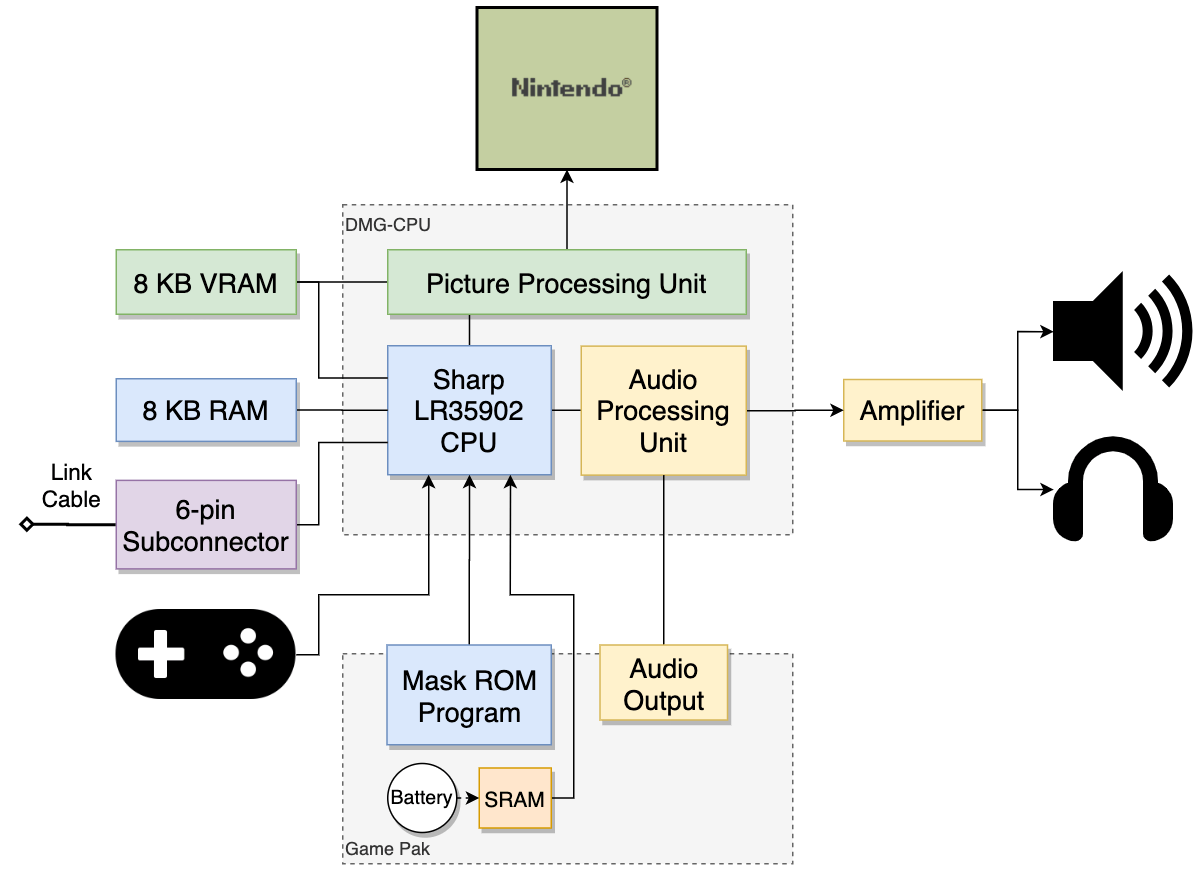
\includegraphics[scale=0.35]{figures/gbdiagram.png}
    \caption{Diagram of the architecture of the Game Boy and the general architecture of a game cartridge (Game Pak). From \cite{gameboyarchitecture}. CC BY 4.0.}
    \label{fig:GameBoyArch-fig}
\end{figure}


%; 8kb RAM; 8kb VRAM; a $160 \times 144$ pixels small LCD, which can display four shades of grey (green on the DMG-01); audio output; a game link port, used to connect multiple Game Boys; buttons for controller input and finally a slot for the game cartridges \cite{gameboyarchitecture}.



\section{Purpose}
%The task is to program an emulator application that can read the ROM extracted from an old console game cartridge, and emulate the hardware that would run the data contained in it, displaying the graphical output the hardware would have, and providing remapped input to the user to interact with the buttons that were in the hardware, allowing them to play the game. Focus will be to have a graphical interface working, not taking sound or other systems into account. The development will suitably take place in C++. The focus is on programming the emulation for the low-level hardware.
The purpose of this thesis is to explore the possibility of emulating a set of microcontrollers which can be assembled to a complete complex system. This is done through emulating the original Game Boy from 1989. In turn, this presents additional purposes as a problem with older gaming consoles is that many of them are no longer produced and are therefore becoming harder and harder to come by. An emulator solves this problem by letting people play old console games on newer hardware. An additional purpose of this thesis is therefore to create a Game Boy emulator for the PC to allow future generations to have the same experience as the people playing the games on the original console whilst also preserving a piece of history. Additionally, the authors would like to share the accumulated knowledge of emulator development with others by providing documentation for the design as well as the code, so that others may learn from it and possibly use it as a base for their own emulators.

\section{Delimitations}
\label{sec:Delimitations}
To reduce the complexity and scope of this thesis certain delimitations have been made.
The emulation has been limited to only emulate the original Game Boy from 1989 and subsequent with equivalent hardware. This reduces the complexity of the thesis significantly as it reduces the amount of different systems and chips needed to be researched. Furthermore, it also means that the hardware which is to be researched is older and therefore of lower complexity than more modern hardware.
\\\\
Regarding some features and systems in the Game Boy, further limitations are made. First of all; ``Serial Data Transfer'' is not supported. This is a feature which is used to connect a Game Boy to another Game Boy to, amongst other things, allow for multiplayer gameplay \cite{GBWikiSerialDataTransferTutorial}. Although this could be implemented in software by connecting two instances of the emulator on the same machine, or even separate machines, this is simply out of scope and creates too little value for the effort.
%The only kind of hardware port that is regarded in this emulator is the one where you insert your games.
\\\\
The games for the Game Boy comes in cartridges called Game Paks \cite{gamepak}. The specifications of these can differ between different games with a total of 28 different configurations supported by the console, including six different memory bank controllers (MBCs) \cite{cartridgeType}. The aim was not to support all of the configurations, but rather the most significant types. \\\\
The Game Boy also has a feature called ``Vin'', allowing the use of external audio hardware located in the cartridge. However, none of the games made for Game Boy uses this feature \cite{pandDocsSoundControlRegisters} and is therefore excluded from being implemented in the emulator.

\section{Ethics}
\label{sec:introEthics}
Creating an emulator for a previously commercially sold product comes with complications. Because of Nintendo having created the Game Boy, it is natural that they are committed to making sure no one infringes the copyrights related to their product. When discussing emulators, there is also often a discussion of what is right and wrong, what counts as piracy and what is legal to do around the subject of copyright. 
\\\\
Nintendo Australia  states the following regarding emulators \cite{NintendoCopyright}:
\\\\
\textit{\textbf{"A Nintendo emulator is a software program that is designed to allow gameplay on a platform that it was not created for. A Nintendo emulator allows for Nintendo console based or arcade games to be played on unauthorised hardware. The video games are obtained by downloading illegally copied software, i.e. Nintendo ROMs, from Internet distributors. Nintendo ROMs then work with the Nintendo emulator to enable game play on unauthorised hardware such as a personal computer, a modified console, or another video game device."}}
\\\\
Thereby Nintendo are neither stating that the use of emulators per se, nor that the development of them is illegal as long as no copyrighted material is used. They do however claim that the games that are used together with emulators are obtained illegally. All of this leads to a lot of confusion around the legality and ethics of emulation, further discussion regarding this topic can be found in section \ref{sec:Ethics}.

%in one of Nintendo's website's legal pages, they do not mention emulators themselves to be illegal, however instead claim that the games that are used with emulators are obtained illegally. All of this leads to huge confusion around the legality and ethics of emulation, which will be further discussed in this report.
%https://www.nintendo.com.au/legal

%Ingen officiell dokumentation -> svårare att utveckla. Hade det funnits had det funnits risk att man uppmanade copyright infringements. - Done

% THEORY
\chapter{Theory}
\label{chap:Theory}
%This section documents the hardware of the Game Boy which must be emulated.

This section aims to describe the various components used in the Game Boy. This is needed to then be able to understand how to properly emulate the function of those components.

\section{The Central Processing Unit}
The Central Processing Unit (CPU) used in the Game Boy is a Sharp LR35902 \cite{pandoscspecifications} \cite{gameboyhistory} which is designed specifically for the Game Boy. The chip is heavily inspired by the Zilog Z80 \cite{Z80} and the Intel 8080 \cite{Intel8080}. While the CPU itself has a clock frequency of 4 MHz \cite{pandoscspecifications}, one can consider it having an actual clock speed of 1 MHz. 
This is due to the fact that the CPU is bound by the speed of the memory \cite{GBTClockSpeed} (the rate the RAM can provide data to the CPU) which has a clock speed of 1 MHz, see slide 149 of  \cite{ultimateGBtalkSlides}. 
%see slide 149
%In addition to this, the CPU is most probably following the fetch-decode-execute cycle, making a machine cycle equal to that of four clock cycles.
Furthermore, the CPU has a 16-bit address bus \cite{pandocsmemorymap} and an 8-bit arithmetic logic unit (ALU).
\subsection{Registers}
The CPU has six general purpose registers, B, C, D, E, H and L \cite{pandocsregistersandflags}. These are all 8 bits each, but can be used pairwise as three 16-bit registers, BC, DE and HL. There are also two additional 8-bit registers, A and F, which both have specific purposes. A is the accumulator register where all the arithmetic is done. The F register, despite being 8 bits, only uses 4 bits to store the value of the four flags of the ALU. These are the zero, negative, half-carry and carry flags \cite{pandocsregistersandflags}, abbreviated as Z, N, H and C respectively. Additionally, the CPU has a 16-bit program counter (PC) and stack pointer (SP).

\subsection{Instruction set}
In total the CPU supports 500 assembly instructions, of which 244 are 8-bit and 256 are 16-bit, see Figure \ref{fig:8bitOpCodes} for the 8-bit instructions. For the CPU to interpret the 16-bit operations, a certain prefix is used (\texttt{0xCB}) found in the 8-bit table allowing the CPU to interpret the following 8 bits as an instruction from the 16-bit table. The tables specify for each instruction which flags it affects, how many bytes it is encoded with and how many machine cycles it requires to execute. 
\\\\
\begin{figure}[H]
    \centering
    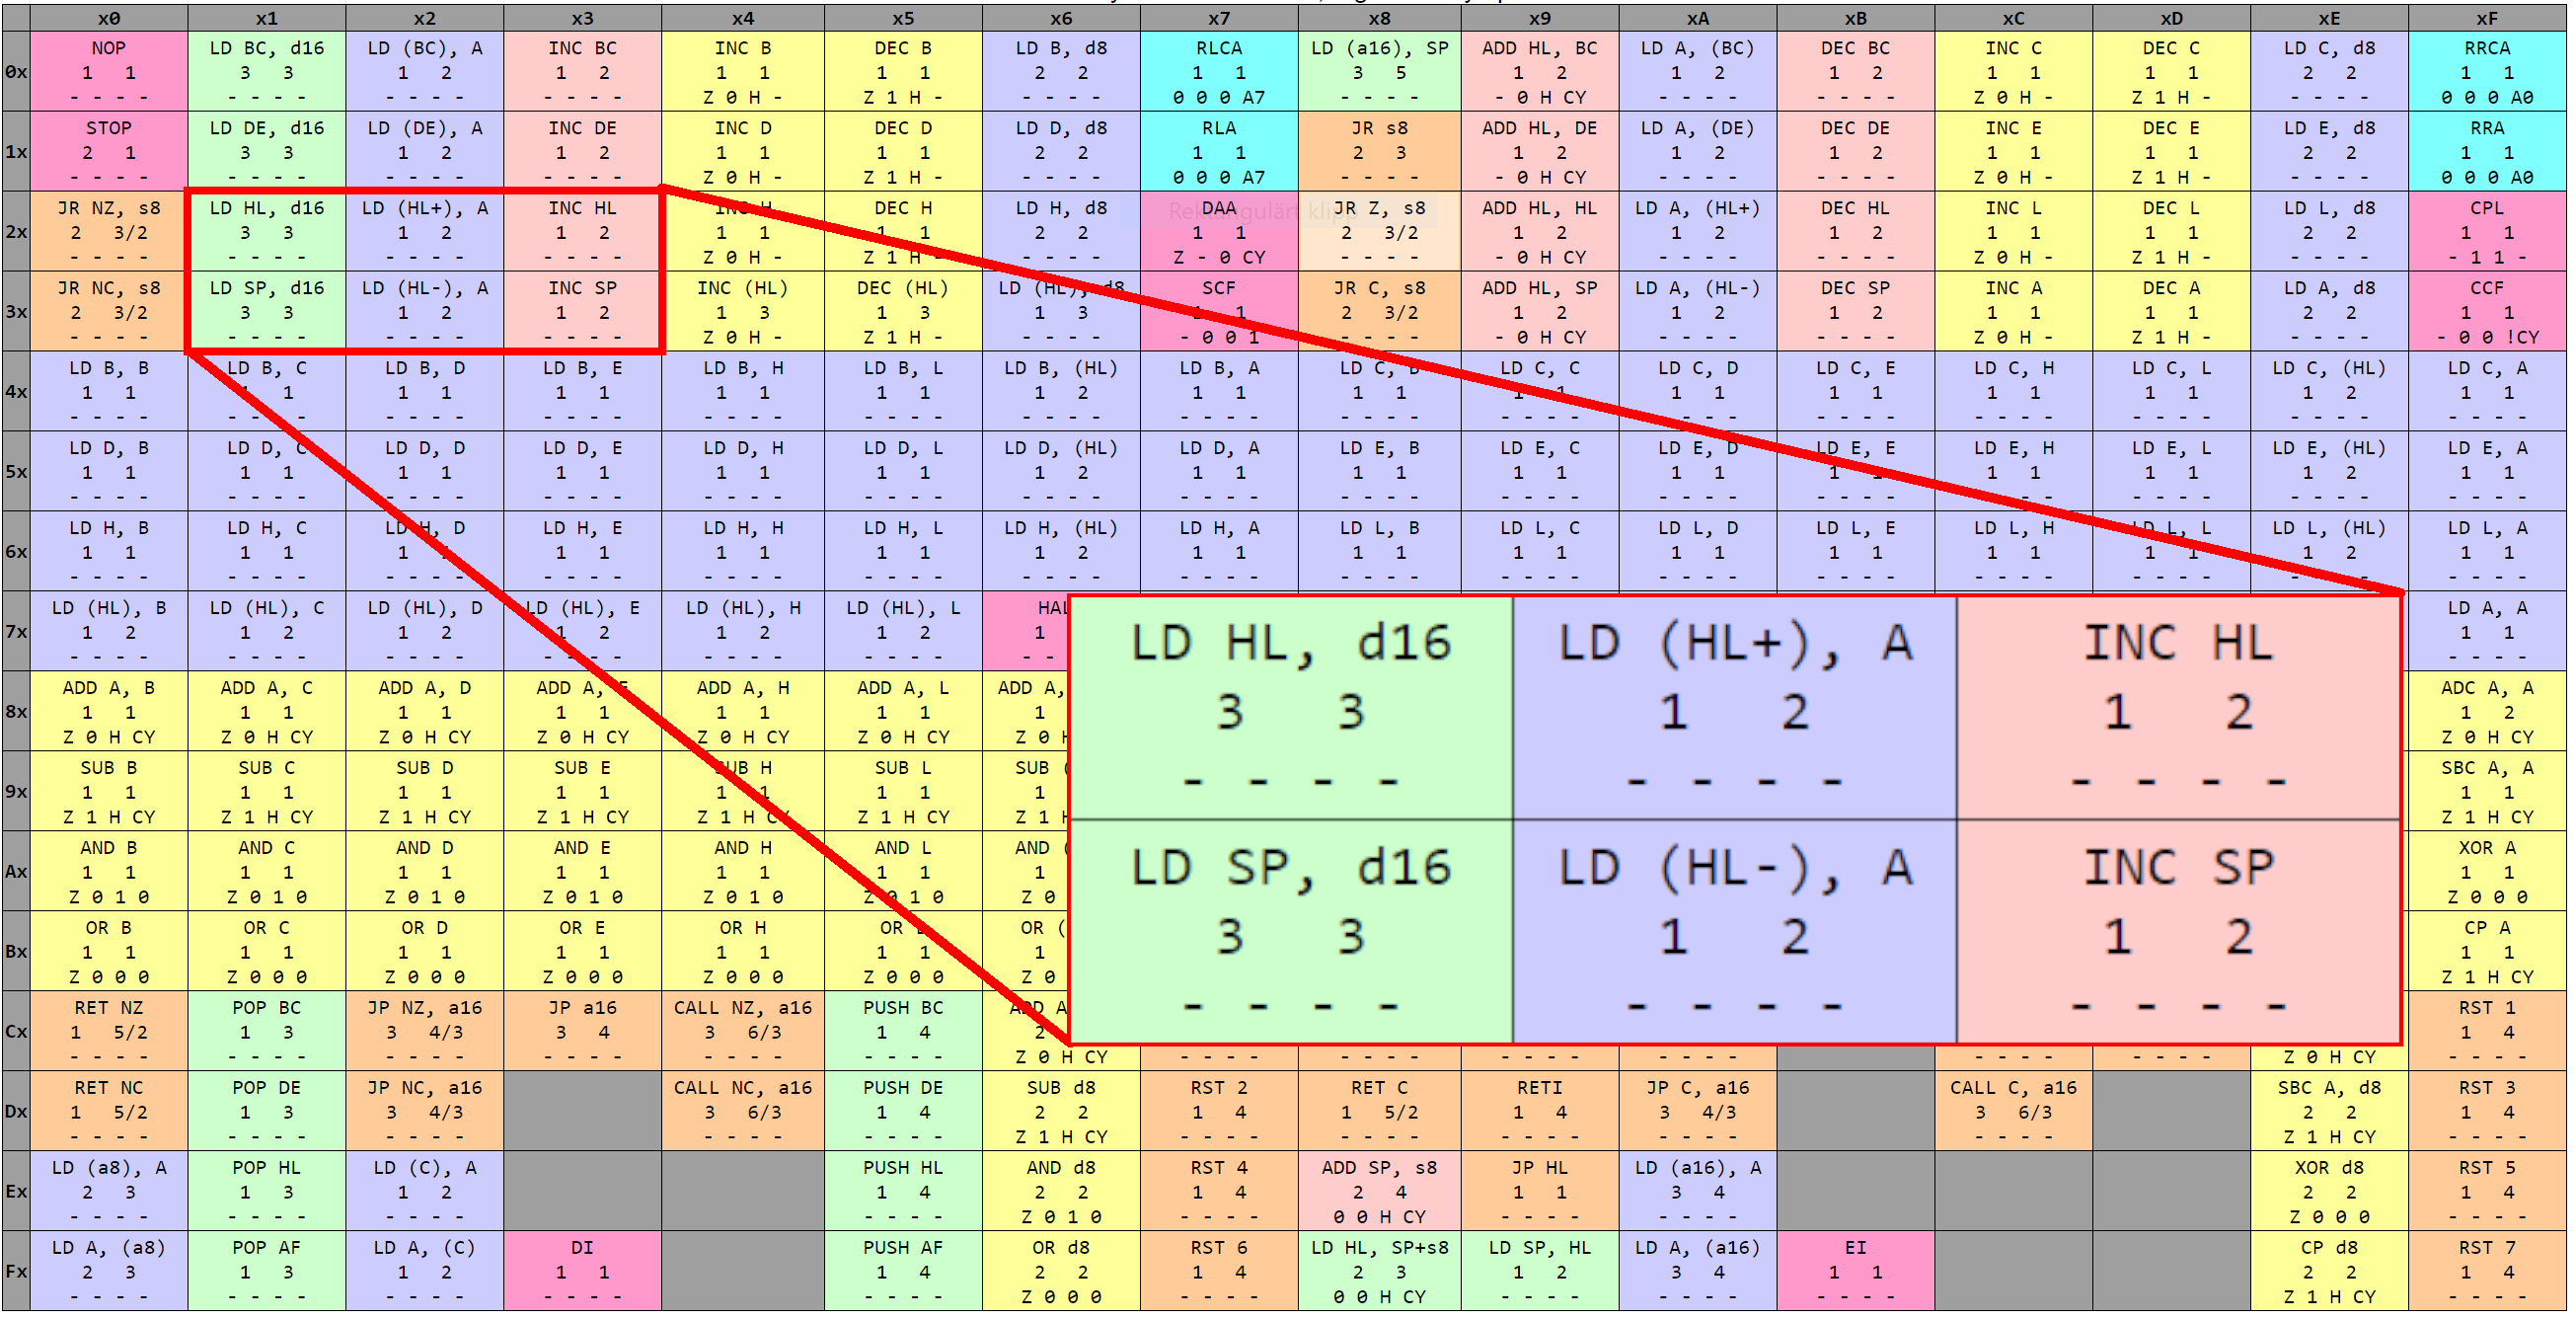
\includegraphics[width=\textwidth]{figures/8bitOpCodes.PNG}
    \caption{Displaying the 8-bit operation codes for the LR35902, highlighting six of the operation codes, showing their assembly instruction, number of bytes used, number of cycles to execute and what flags are affected. From \cite{OpCodes}. Modified with permission.}
    \label{fig:8bitOpCodes}
\end{figure}


%\begin{figure}[H]
%    \centering
%    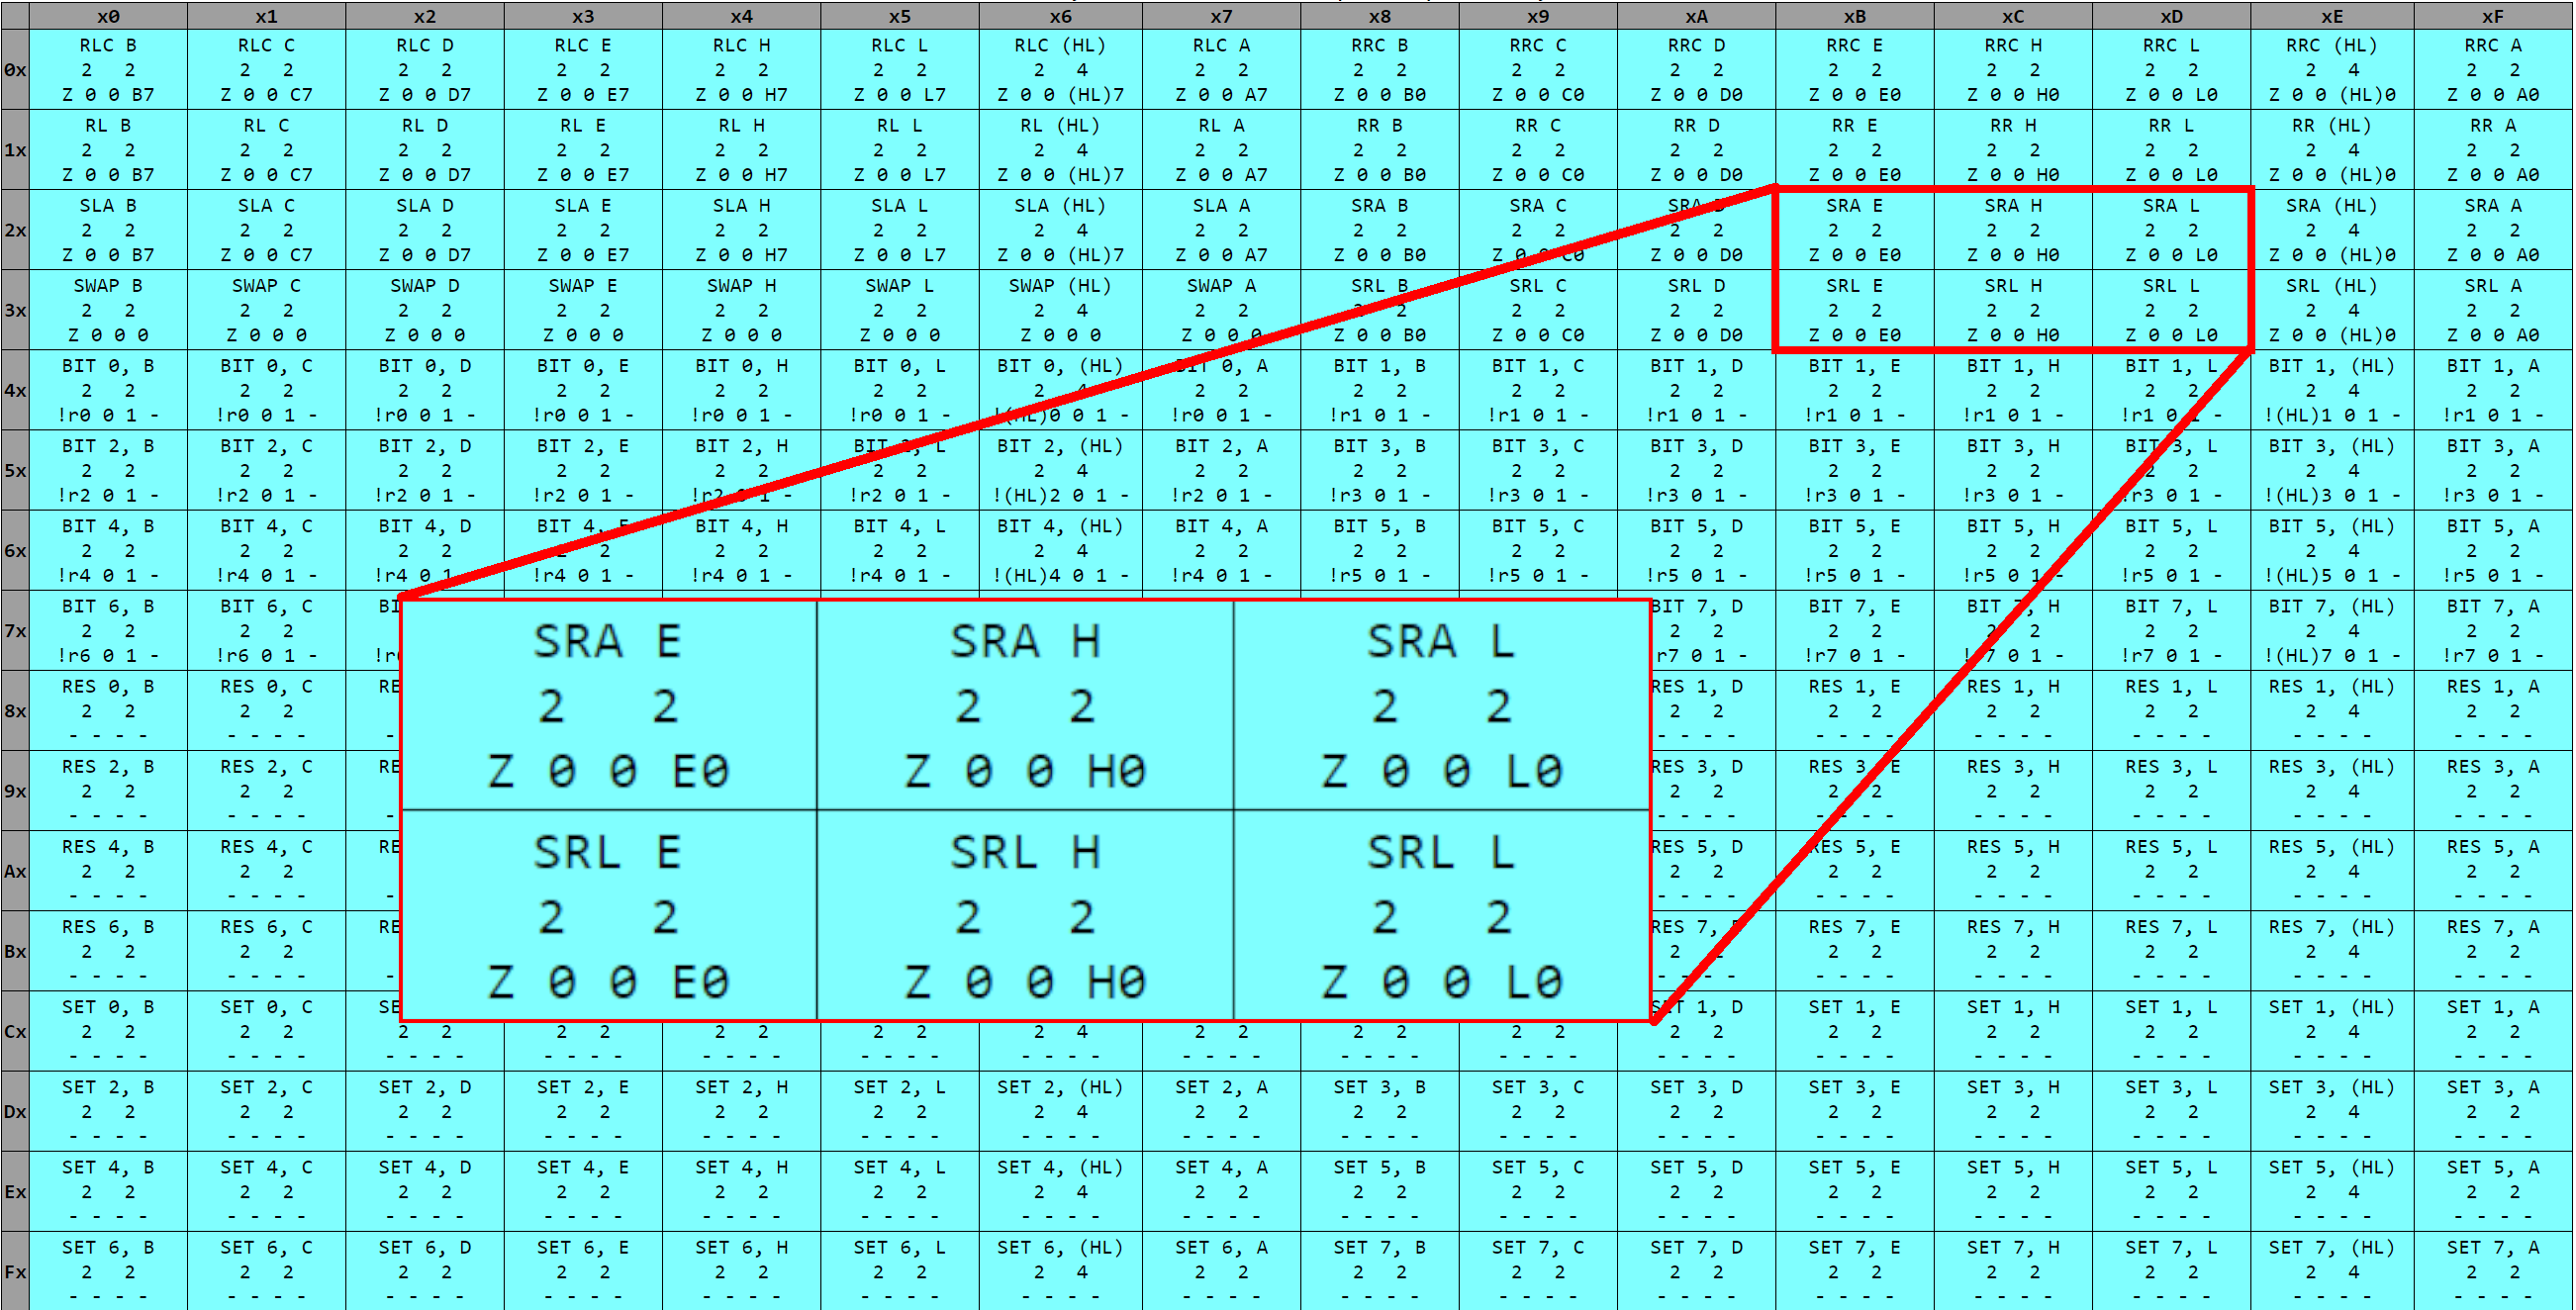
\includegraphics[width=\textwidth]{figures/16bitOpCodes.PNG}
%    \caption{Displaying the 16-bit operation codes for the %LR35902, highlighting six of the operation codes, showing their %assembly instruction, number of bytes used, number of cycles to %execute and what flags are affected. From \cite{OpCodes}. %Modified with permission.}
%    \label{fig:16bitOpCodes}
%\end{figure}
\subsection{Interrupts}
\label{sub}

Like many other CPUs, the Sharp LR35902 supports interrupts. Interrupts are used in order to break the regular flow of the CPU, forcing it to handle the interrupt before returning to what it was doing previously.
%The interrupts are handled by the CPU by continuously checking a number of bits and whether or not they are set.
Different interrupts have different pre-defined addresses where the respective interrupt routines are stored \cite{pandocsinterrupts}. When an interrupt occurs, the CPU executes the interrupt routine, and then continues execution from the address that was current when the interrupt occurred. The existing interrupts and their functionalities are the following \cite{pandocsinterrupts}:
\\
\begin{itemize}
    \item V-blank - An interrupt sent from the PPU when it has created a whole frame and wants to draw it, for more information see Section \ref{sec:PPU}.
    \item LCD STAT - A customisable interrupt regarding various conditions of the PPU. An interrupt is generated any time the PPU goes from not meeting any condition to meeting at least one condition. Which conditions are used is determined by the STAT register of the PPU, for more information, see Section \ref{sec:PPU_Registers}
    \item Timer - Sends an interrupt request when a set timer has run out, for more information see Section \ref{sec:Timer}.
    \item Serial - The serial transfer interrupt which handles the communication between two Game Boys when they are connected through the serial port. This is not implemented, as is explained in Section \ref{sec:Delimitations}.
    \item Joypad - An interrupt which handles the input from the joypad, for more information see Section \ref{sec:Joypad}.
    \\
\end{itemize}

The interrupts are implemented by having three different types of flag registers \cite{pandocsinterrupts}:
\begin{itemize}
    \item IME - Interrupt Master Enable. This flag enables and disables all other interrupt flags. Can only be manipulated through specific instructions.
    \item IE - Interrupt Enable. Enables or disables a specific flag. Consists of five bits, one for each type of interrupt. Manipulated through memory, located at \texttt{0xFFFF}.
    \item IF - Interrupt Flag. Shows that an interrupt has been requested. This is the flag which is set when an interrupt is raised. The register consists of five bits, one for each type of interrupt. Manipulated through memory, located at \texttt{0xFF0F}.
    \\
\end{itemize}
If IME is disabled, IE and IF can still be altered, but they are not acted upon until IME is enabled once again. For an interrupt to occur and be handled by the CPU three things therefore need to happen: both the IME flag and a specific IE flag must be enabled, and the corresponding IF flag must be triggered \cite{pandocsinterrupts}. 
\\\\
\newpage
\section{Memory and I/O devices}
\label{sec:MMUTheory}
The CPU needs to access memory and communicate with peripheral devices. To achieve this the Game Boy uses a 16-bit address bus and an 8-bit data bus \cite{TCAGBD}. The memory and different peripheral devices are mapped to specific memory addresses visualised in Figure \ref{fig:memory-map}.

%\begin{figure}[H]
%    \centering
%    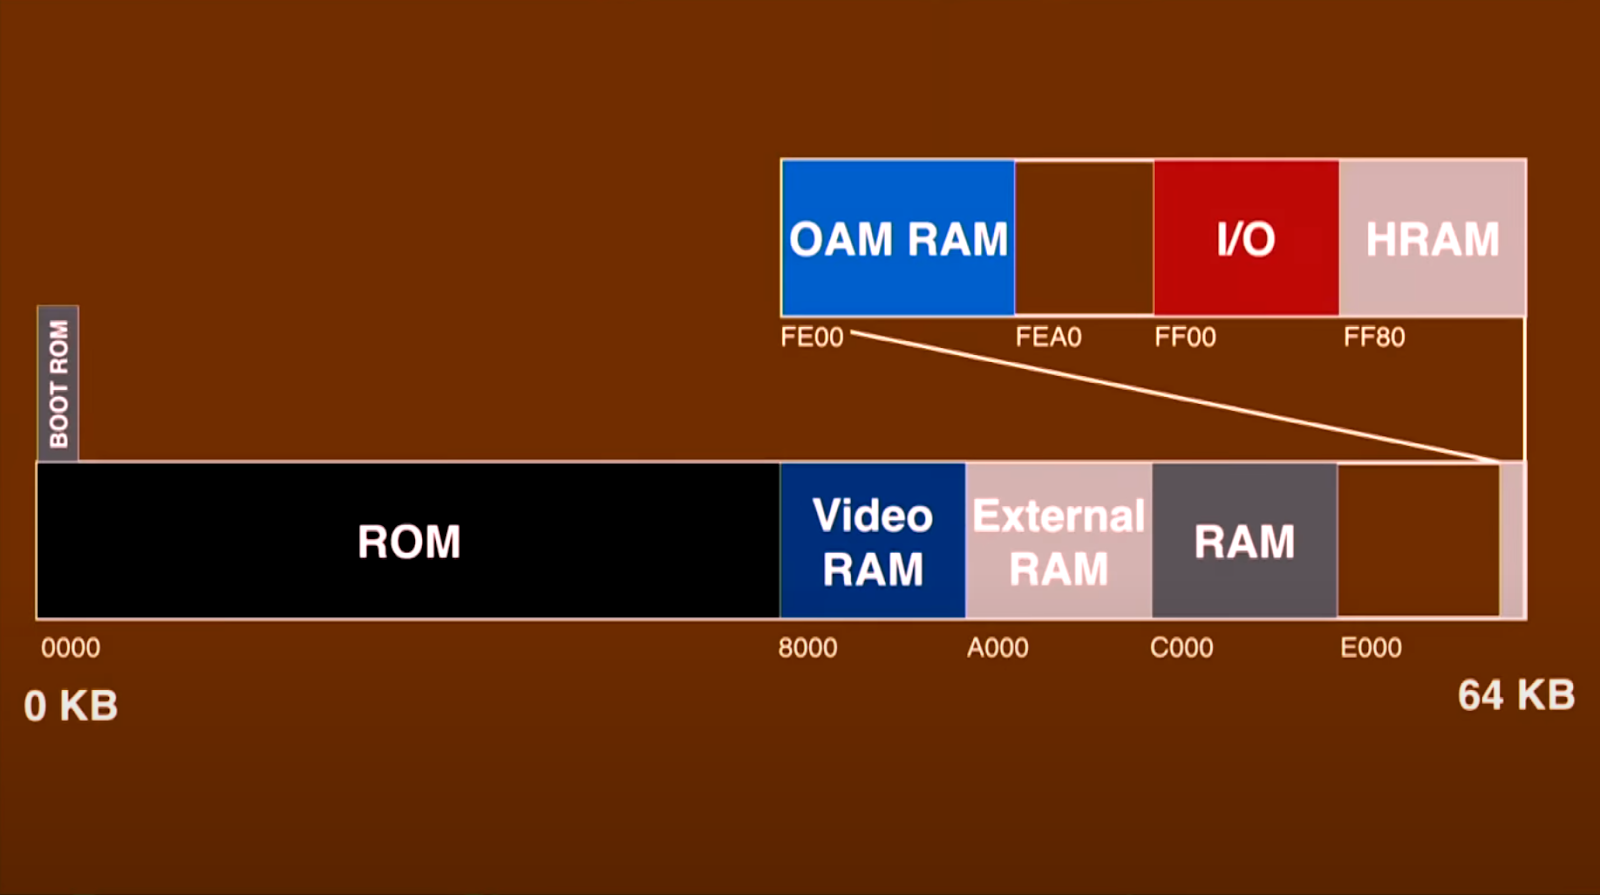
\includegraphics[scale=0.25]{figures/Memory.png}
%    \caption{Visual representation of how the address space is divided in the Game Boy \cite{GBTMem}.}
%    \label{fig:memory-map}
%\end{figure}

\begin{figure}[H]
    \centering
    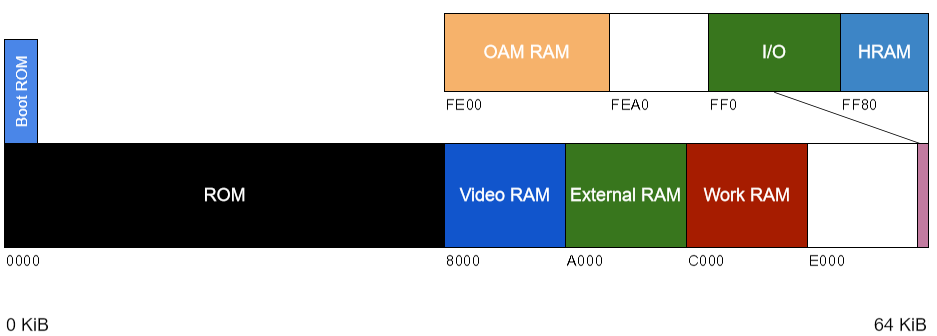
\includegraphics[width=\textwidth]{figures/Memory Map.PNG}
    \caption{Visual representation of how the address space is divided in the Game Boy. From \cite{ultimateGBtalkSlides}. Adapted with permission.}
    \label{fig:memory-map}
\end{figure}
In the Game Boy's 64 KiB address space, different address ranges are used for different purposes. Below is a description of how this is handled. Note that the I/O devices are controlled through manipulating address space and that the more complex I/O devices, the PPU and APU, are described in Section \ref{sec:PPU} and Section \ref{sec:APU} respectively.

\subsection{Boot ROM}
\textbf{Address: \texttt{0x00} - \texttt{0xFF}}

The boot ROM is a 256 byte ROM located on the DMG-CPU and contains the code that is executed when the Game Boy is powered on \cite{BootRom}. The purpose of the boot ROM is to initialise the different hardware units and prepare the Game Boy to execute game code \cite{bootstraptechopedia}. The official boot ROM used on the Game Boy does this while scrolling down the Nintendo logotype. The use of copyrighted material on the boot ROM has legal implications which is further discussed in Section \ref{sec:Ethics}.
In practice the boot ROM is only accessible a short time when the Game Boy is powered on due to the fact that it disables itself after it has been run. 
Disabling the boot ROM is done by storing a non-zero value at memory address \texttt{0xFF50} and will map the addresses to the ROM instead, see the overlap in Figure \ref{fig:memory-map}.
\newpage
\subsection{ROM}
\textbf{Address: \texttt{0x0000} - \texttt{0x7FFF}}
\\
The ROM located in the Game Boy's memory map is the area where the interactions with data from the inserted game ROMs happen \cite{pandocsmemorymap}. 
Although the allocated size for the ROM on the Game Boy is only 32 KiB, the ROMs it supports can be much larger. This is possible through the use of bank switching using a Memory Bank Controller (MBC) \cite{pandocsexternalmemoryandhardware}, located in the Game Pak ROM, see Section \ref{sec:MBC} for more information.

\subsection{Video RAM}
\textbf{Address: \texttt{0x8000} - \texttt{0x9FFF}}
\\
The Video RAM (VRAM) is an 8 KiB RAM \cite{pandocsmemorymap} that is accessible by both the CPU and PPU. 
It it used by the CPU to store data which the PPU uses for drawing. 
While the PPU is drawing, it is reading from the VRAM and the CPU is therefore not allowed access. 
For more information regarding how the VRAM is used, see Section \ref{sec:PPU}.


\subsection{External RAM}
\textbf{Address: \texttt{0xA000} - \texttt{0xBFFF}}
\\
The external RAM (XRAM) is an optional memory that is located on some of the game cartridges. Its size varies from game to game and can, if desired, also make use of bank switching (see Section \ref{sec:MBC}). The XRAM is often used for saving progress and high score tables \cite{pandocsmemorymap}. This is done by powering the XRAM with a small battery inside the game cartridge to make sure the data is conserved between different gaming sessions. 
\subsection{WRAM}
\textbf{Address: \texttt{0xC000} - \texttt{0xDFFF}}
\\
The Work RAM (WRAM) is the main memory of the system which is used by the CPU to store any data the game uses while running. The WRAM is located on the DMG-CPU and has a size of 8 KiB \cite{pandocsmemorymap}.


\subsection{OAM RAM}
\textbf{Address: \texttt{0xFE00} - \texttt{0xFE9F}}
\\
The Object Attribute Map (OAM) is the area where sprite data is stored. The OAM is divided into 40 blocks of four bytes each with each block corresponding to a sprite. Both the PPU and CPU have direct access to this memory area. While the PPU is rendering scanlines, the CPU has limited access to this area \cite{pandocsoam}. The CPU can also transfer data into the OAM through the use of Direct Memory Access (DMA) transfers, this process is described in detail in Section \ref{sec:DMA_transfer}.

%There is another way for the CPU to transfer data into OAM: Direct Memory Access (DMA) transfers. This process is described in detail in section \ref{sec:DMA_transfer}.



%\subsection{I/O devices}
%\textbf{Address: 0xFF00 - 0xFF7F}

%The I/O devices are controlled through reading and writing to their control and status registers.
%The more complex I/O devices, the PPU and APU are describes in their own chapters \ref{sec:PPU} and \ref{sec:APU} respectively. In this chapter the Joypad and the Timer will be described.
\subsection{Joypad}
\label{sec:Joypad}
%\subsubsection{Joypad}
\textbf{Address: \texttt{0xFF00}}
\\
The Joypad is the device that connects the user's input with the system. 
There are eight buttons on the Game Boy, four directional buttons: up, down, left and right, and four action buttons: A, B, Start and Select.
The buttons have two states, pressed or not pressed. 
These states of the buttons are stored at address \texttt{0xFF00} as a 2x4 matrix \cite{pandocsjoypad}.
\\\\
By writing specific values to bit 4 and 5 either the action buttons or directional buttons will be selected.
When selecting either the action or direction buttons bit 0-3 will correspond to the selected buttons \cite{pandocsjoypad}. See Table \ref{tab:joypad}.


\begin{table}[H]
    \begin{center}

\begin{BVerbatim}
Bit 7 - Not used
Bit 6 - Not used
Bit 5 - Select Action buttons    (0=Select)
Bit 4 - Select Direction buttons (0=Select)
Bit 3 - Input: Down  or Start    (0=Pressed) (Read Only)
Bit 2 - Input: Up    or Select   (0=Pressed) (Read Only)
Bit 1 - Input: Left  or B        (0=Pressed) (Read Only)
Bit 0 - Input: Right or A        (0=Pressed) (Read Only)
\end{BVerbatim}

    \caption{Layout of the button states located in memory address \texttt{0xFF00}. From \cite{pandocsjoypad}. Adapted with permission.}
    \label{tab:joypad}
    \end{center}
\end{table}

When a button is pressed, an interrupt is raised, but only if the pressed button is a button that is selected by bit 4 and 5 (either an action or a directional button) \cite{pandocsjoypad}. Regarding how to actually handle the joypad input, it is up to the developer to either poll the $2 \times 4$ -matrix or by using the interrupts.

\subsection{Timer}
\label{sec:Timer}
%\subsubsection{Timer}

\textbf{Address: \texttt{0xFF04} - \texttt{0xFF07}}

The Game Boy has a built-in timer which can be used to perform time sensitive tasks. 
It is used and controlled by reading and writing to the following registers \cite{pandocstimer}:
\\\\
\textbf{Divider Register - DIV}
\\
\textbf{Address: \texttt{0xFF04}}
\\
The DIV register is a counter that always increments at a rate of 16384Hz. 
When writing any value to the address the counter resets to 0 \cite{pandocstimer}.
\\\\
\newpage
\textbf{Timer counter - TIMA}
\\
\textbf{Address: \texttt{0xFF05}}
\\
This is another counting register, it increments at the rate that is specified in the TAC register. 
When the counter value is 0xFF and overflows it is reset to the value in TMA as the new counter value.
When the counter overflows the ``Timer''-interrupt is raised \cite{pandocstimer}.
Writing to this register simply changes the counter to the written value.
\\\\
\textbf{Timer Modulo - TMA}
\\
\textbf{Address: \texttt{0xFF06}}
\\
This register holds the timer modulo value.
This value is loaded into the TIMA register when the TIMA counter overflows \cite{pandocstimer}.
It can be used to further modify the chosen clock speed chosen in the TAC register.
\\\\
\textbf{Timer Control - TAC}
\\
\textbf{Address: \texttt{0xFF07}}
\\
This register is used to control the timer.
By writing to this register the timer can be enabled or disabled. The rate at which the TIMA register will increment can also be controlled by writing to this register \cite{pandocstimer}. 
\\\\
As shown in Table \ref{tab:timer_tac}, bit 2 enables or disables the timer. 
Notice that disabling the timer does not stop the DIV counter.
Bits 0 and 1 are used to select one out of four possible clock speeds; 4069 Hz, 262144 Hz, 65536 Hz or 16384 Hz \cite{pandocstimer}. 

\begin{table}[H]
    \begin{center}

\begin{BVerbatim}
Bit  2   - Timer Enable
Bits 1-0 - Input Clock Select
           00: CPU Clock / 1024 (4096 Hz)
           01: CPU Clock / 16   (262144 Hz)
           10: CPU Clock / 64   (65536 Hz)
           11: CPU Clock / 256  (16384 Hz)
\end{BVerbatim}

    \caption{Layout of the each bit in the timer control register located at address \texttt{0xFF07}. From \cite{pandocstimer}. Modified with permission.}
    \label{tab:timer_tac}
    \end{center}
\end{table}

\subsection{HRAM}
\textbf{Address: \texttt{0xFF80} - \texttt{0xFFFE}}

The high RAM or HRAM is very much like the WRAM although it is much smaller and faster to access. 
It is faster because of a special instruction that assumes that the highest byte in the address is \texttt{0xFF} and therefore saves time decoding the instruction \cite{OpCodes}. 
During a DMA-transfer (see Section \ref{sec:DMA_transfer}) the CPU is limited to use only this memory.
The size of the HRAM is 126 bytes \cite{pandocsmemorymap}. 
\newpage
\subsection{Memory Bank Controllers}
\label{sec:MBC}
As previously mentioned, the Game Boy uses a 16-bit address bus, which in turn limits the memory addresses available for the game ROM and external RAM. 
To bypass this limitation many game cartridges make use of a memory bank controller (MBC).
The MBC is used to map different sections of a memory, called memory banks, to one specific address range, this method is called bank switching.
It works as follows: reading from addresses \texttt{0x0000} to \texttt{0x7FFF} returns a byte stored on the ROM as expected, but writing to those same addresses will instead change the MBC's control registers, this is further described below and in Figure \ref{fig:MBC3}. 
These control registers control what memory bank is to be used for both the game ROM and the external RAM (if any).
\\\\
There are different versions of MBCs which all support various arrangements of additional hardware. 
Examples of such hardware are external RAM with or without a battery powering said RAM and in some cases also a timer \cite{GBWikiMBC}. For example, MBC3 supports up to 2 MiB of ROM and/or 64 KiB of RAM, and Real Time Clock (RTC) with battery \cite{GBWikiMBC}.

\begin{figure}[H]
    \centering
    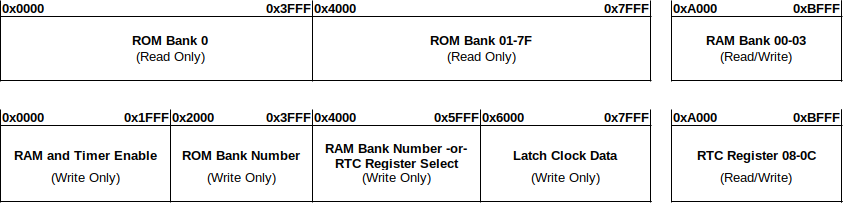
\includegraphics[scale=0.5]{figures/MMU/MBC3_figure_no_padding.png}
    \caption{Memory map of MBC3. While all MBCs do not necessarily contain the same features, most follow a similar structure \cite{GBWikiMBC}.}
    \label{fig:MBC3}
\end{figure}

The following is a description of the structure and functionality of MBC3, shown in Figure \ref{fig:MBC3} \cite{GBWikiMBC}:
\\\\
\textbf{ROM Bank 0 }
\\
Contains the first 16 KiB of the ROM.
\\\\
\textbf{ROM Bank 0x01-0x7F}
\\
This part of the memory is used for bank switching. There are at most 127 available memory banks each with a size of 16 KiB, resulting in a total ROM size of $128 \times 16$ KiB = 2 MiB, including ROM bank 0.
\\\\
\textbf{RAM and Timer Enable}
\\
Writing specific values to this address will enable reading and writing to XRAM or RTC registers depending on which is currently active.
\\\\
\textbf{ROM Bank Number}
\\
Writing to this address controls which ROM bank is in use.
\\\\
\textbf{RAM Bank Number/RTC Register Select}
\\
Writing to this area maps the corresponding XRAM bank or RTC register into the memory of \texttt{0xA000}-\texttt{0xBFFF}. 
\\\\
\textbf{RAM Bank 0x00-0x03 or RTC Register 0x08-0x0C}
\\
Depending on the current \textbf{Bank Number/RTC Register selection}, this memory space is used to either access an 8 KiB external RAM Bank, or a single RTC Register, see Table \ref{tab:rtc_registers}.
\\\\
\textbf{Latch Clock Data}
\\
If writing first 0x00, and then 0x01 to this register, the current time becomes latched into the RTC register. This means that the current time can be read from the register while the RTC continues to tick. Additionally the RTC needs a quartz oscillator as well as an external battery to work while the Game Boy is turned off. 
\\\\
\begin{table}[H]
    \begin{center}

\begin{BVerbatim}
0x8  RTC S   Seconds   0-59 (0x00-0x3B)
0x9  RTC M   Minutes   0-59 (0x00-0x3B)
0xA  RTC H   Hours     0-23 (0x00-0x17)
0xB  RTC DL  Lower 8 bits of Day Counter (0x00-0xFF)
0xC  RTC DH  Upper 1 bit of Day Counter, Carry Bit, Halt Flag
      Bit 0  Most significant bit of Day Counter (Bit 8)
      Bit 6  Halt (0=Active, 1=Stop Timer)
      Bit 7  Day Counter Carry Bit (1=Counter Overflow)
\end{BVerbatim}

    \caption{List of the different RTC registers and its contents. From \cite{pandocsmbc}. Adapted with permission.}
    \label{tab:rtc_registers}
    \end{center}
\end{table}


%\end{comment}

\newpage
\section{The Pixel Processing Unit}
\label{sec:PPU}

The purpose of the Pixel Processing Unit (PPU) is to interpret the data residing in VRAM and compose it into a picture which can then be printed on the LCD. The CPU can communicate with the PPU either by loading data into the VRAM or by reading from or writing to a number of hardware registers, most notably the LCD control and status registers. The PPU, on the other hand, uses interrupts to communicate with the CPU \cite{pandocsVideo}.

\subsection{Composing the frame}
\label{sec:PPU_image}

The frame is composed of three layers: Background, Window and Sprites, rendered in that order. These layers are in turn composed of tiles, 8x8 bitmaps of colour indices, which are stored in VRAM. When rendering the picture, these indices map to one of the four colours using palette tables, which in the original Game Boy was four shades of grey over a green background \cite{gameboyarchitecture}. The following is a description of the components used to form the frame.\\
\\
\textbf{Tiles} - 
As previously mentioned, the tiles are 8x8 bitmaps stored in RAM, 16 bytes per tile. This is because each row of a tile is formed by combining the bits of two bytes. The bytes are organised in two memory regions called \textit{Tile sets}; one ranging from \texttt{0x8000} to \texttt{0x9000} and one ranging from \texttt{0x8800} to \texttt{0x9800}, see Figure \ref{fig:ppu_tile_set}. These two tile sets overlap and which one to use is determined by a bit in the LCD Control register (LCDC). The first of the two uses unsigned addressing for tile IDs, while the second one uses signed addressing. \cite{gameboyarchitecture}.
\newpage
\begin{figure}[H]
    \centering
    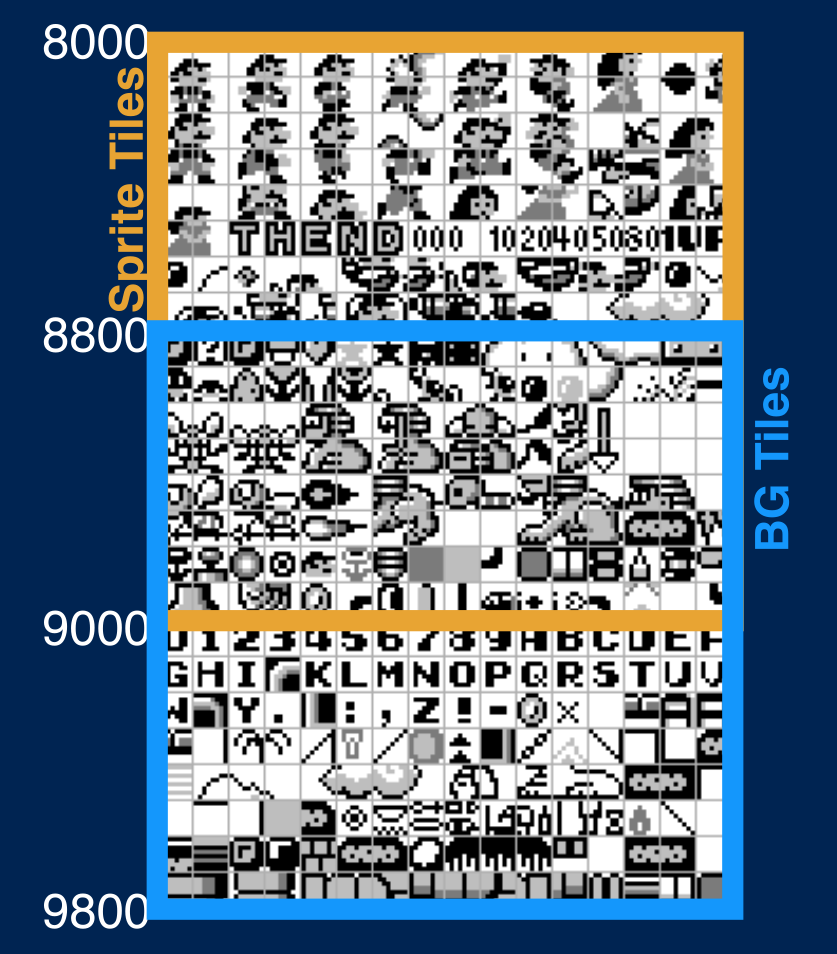
\includegraphics[width=0.8\linewidth]{figures/PPU/PPU_tile_sets_divided.png}
    \caption{The two tile sets. Sprites may only use tiles from the tile set ranging from \texttt{0x8000} to \texttt{0x9000} while the background and window can use any of the two sets. From \cite{ultimateGBtalkSlides}. Used with permission.}
    \label{fig:ppu_tile_set}
\end{figure}
%Slide 434
\textbf{Background} - 
The background is defined by a map of 32x32 tile IDs. Since a tile is 8x8 pixels, this results in a map of 256x256 pixels; however, the Game Boy's display is only 160x144 pixels. The result of this is that only part of the background is being displayed at any given time, as shown in Figure \ref{fig:ppu_viewport}. Which part of the map to display is determined by the two hardware registers, SCX and SCY, which specify which pixel should appear in the top left corner of the display. If the edge of the map is reached, the map loops around and continues at the opposite side. There are also two maps available at any given time, which one is being used is determined by a bit in the LCDC \cite{pandocsVideo}.\\
\\
\begin{figure}[H]
    \centering
    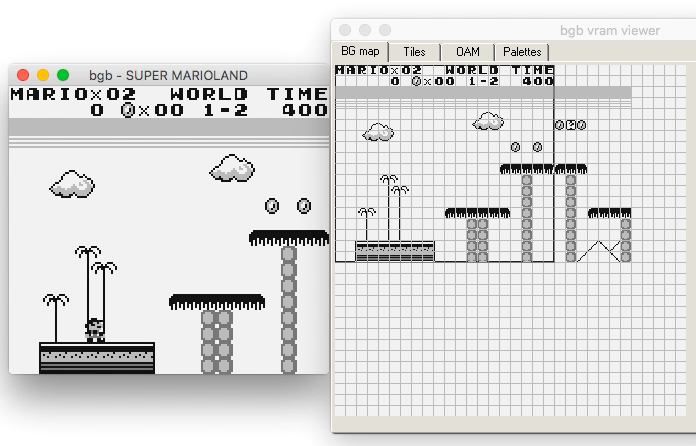
\includegraphics[width=\linewidth]{figures/PPU/PPU_viewport.png}
    \caption{What is shown on the LCD in relation to the background map. From \cite{ultimateGBtalkSlides}. Used with permission.}
    \label{fig:ppu_viewport}
\end{figure}
%Slide 320
\textbf{Window} - 
The window is drawn on top of the background. Just like the background, it consists of a map of tiles; however, this map is only 20x18 tiles, just covering the entire screen and, unlike the background, does not loop around. This layer can be used to display information that should not scroll with the rest of the background, such as a GUI \cite{pandocsVideo}.\\
\\
\textbf{Sprites} - 
Sprites are objects that can move around on the screen freely. They consist of one or two tiles, depending on a bit in the LCDC register. As opposed to the tiles in the background and window layers, sprites can have transparent pixels, meaning that the background and window are still visible through said pixels. Sprites only consist of tiles from the tile set ranging from \texttt{0x8000} to \texttt{0x9000}, as shown in Figure \ref{fig:ppu_tile_set} \cite{pandocsVideo}.\\
\\
Sprite data is stored in a memory region called the Object Access Map(OAM). Each sprite takes up four bytes of memory. These bytes store the sprites' x and y coordinates, the sprites' tile IDs and a set of flags. The flags describe which of two object palettes the sprite uses, whether the sprite is flipped horizontally or vertically, and lastly whether the sprite should be drawn in front of or ``behind'' the background. Drawing a sprite ``behind'' the background results in background and window pixels with colour indices 1-3 being drawn in front of the sprite, though the sprite is still drawn in front of pixels with colour index 0 \cite{pandocsVideo}.

\subsection{The modes}
\label{sec:PPU_Modes}
At any given time, the PPU is in one of four modes: horizontal blanking, vertical blanking, OAM search or drawing \cite{pandocsVideo}.

\begin{figure}[H]
    \centering
    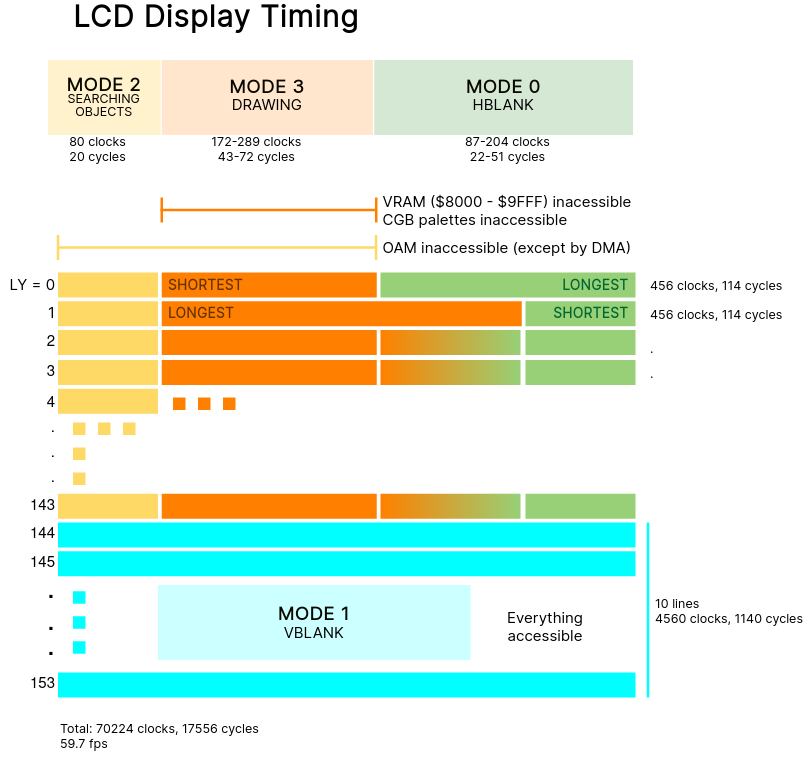
\includegraphics[scale=0.5]{figures/PPU/Mode_diagram.png}
    \caption{The various PPU modes and their durations. From \cite{pandocs}. Public Domain.}
    \label{fig:PPU_timing}
\end{figure}

Depending on which mode the PPU is in, there are limits on whether the CPU has direct access to VRAM and OAM. When the CPU does not have access to one of these regions, any write to that region will be ignored and any read will return 0xFF. The PPU changes modes according to Figure \ref{fig:PPU_timing} \cite{pandocsVideo}. The four modes will now be described in further detail.\\
\\
\textbf{Horizontal blanking}
\\
The PPU enters a horizontal blank (H-blank) whenever it has finished drawing a line. During this period, the CPU can access VRAM and OAM freely. Depending on how long the PPU was in mode 3 before entering this mode, the length of the H-blank is adjusted so that the total time spent on OAM search, drawing and H-blanking for each line is exactly 114 cycles \cite{pandocsVideo}.\\
\\
\textbf{Vertical blanking}

The PPU enters a vertical blank (V-blank) whenever all 144 scanlines have been drawn to the screen. The V-blank is treated as ten blank lines and therefore lasts for 1140 cycles. During this time the CPU has free access to VRAM and OAM \cite{pandocsVideo}.\\
\\
\textbf{OAM search}

The PPU enters this mode before drawing each line. When in this mode, the PPU finds the first ten sprites in OAM that intersect the current scanline to prepare for the draw phase. During this time the CPU can access VRAM freely \cite{pandocsVideo}. \\
\\
\textbf{Drawing}

The PPU enters this mode after having finished OAM search. During this mode the PPU combines the background, window and sprites of the current row and draws the pixels to the LCD. The process is described in more detail in Section \ref{sec:PPU_Drawing}. During this time the CPU can access neither VRAM nor OAM \cite{pandocsVideo}. 

\subsection{The registers}
\label{sec:PPU_Registers}

The PPU contains a variety of hardware registers. These are described in this section, also noting whether they are used for reading or writing to. \\
\\
\textbf{LCD Control Register (R/W)}\\
The LCDC register is the main way for the CPU to control the operation of the PPU. It can be modified at any time and contains the following bits \cite{pandocsLCDC}:\\
\\
\begin{itemize}
    \item Bit 7 - LCD enable. If this bit is 0, the display is off.
    \item Bit 6 - Window tile map select. This bit determines which map should be used for the window layer.
    \item Bit 5 - Window enable. This bit determines whether the window layer should be drawn or not.
    \item Bit 4 - Tile set select. This bit determines which tile set should be used by the tile maps.
    \item Bit 3 - Background tile map select. This bit determines which map should be used for the background layer.
    \item Bit 2 - Object size. This bit determines whether sprites consist of one or two tiles.
    \item Bit 1 - Object enable. This bit determines whether sprites should be drawn or not.
    \item Bit 0 - Background and window enable. This bit determines whether the background and window layers should be drawn or not.
\end{itemize}

\vspace{30pt}
\newpage
\textbf{LCD Status and Configuration Register (R/W)}\\
The STAT register represents the status of the PPU. It can also be used to create custom interrupts, depending on the status of the PPU. The STAT register contains the following bits \cite{pandocsSTAT}:\\
\\
\begin{itemize}
    \item Bit 6 - LYC interrupt enable. Enables interrupts when the current scanline equals the value of the LYC register.
    \item Bit 5 - OAM search interrupt enable. Enables interrupts when the PPU enters OAM search.
     \item Bit 4 - V-blank interrupt enable. Enables interrupts when the PPU enters a V-blank.
    \item Bit 3 - H-blank interrupt enable. Enables interrupts when the PPU enters an H-blank.
    \item Bit 2 - LYC=LY flag. Is set to 1 if the current scanline equals the value of the LYC register.
    \item Bit 1-0 - Mode flag. Represents the current mode of the PPU.
\end{itemize}

\vspace{30pt}

The PPU also has a variety of utility registers, described here \cite{pandocsVideo}:\\
\\
\begin{itemize}
    \item SCY and SCX (Scroll X \& Y) - Control background scrolling. Represents the coordinate on the background map that should be displayed in the top left corner of the display. (R/W)
    \item LY (Line Y) - Keeps track of the current scanline. (R)
    \item LYC (Line Y Compare) - Used in the STAT register to generate interrupts. (R/W)
    \item WY and WX (Window X \& Y) - Represents the coordinate on the display where the top left pixel of the window should be displayed. (R/W)
%    \item BGP (Background Palette) - The palette for the background. Maps the colour indices 0-3 to the colours white (0), light grey (1), dark grey (2) and black (3). (R/W)
    \item BGP (Background Palette) - The palette for the background. Maps the indices 0-3 to white (0), light grey (1), dark grey (2) or black (3). (R/W)
    \item OBP0 (Object Palette 0) - The first of two sprite palettes. Functions similarly to BGP except colour index 0 represents transparent pixels. (R/W)
    \item OBP1 (Object Palette 0) - The second of two sprite palettes. Functions exactly like OBP0. (R/W)
    \item DMA (Direct Memory Access) - Used for triggering a DMA transfer. More information can be found in Section \ref{sec:DMA_transfer}.  (R/W)
\end{itemize}
\newpage
\subsection{Drawing the image}
\label{sec:PPU_Drawing}
During mode 3 the PPU continuously transfers pixels to the LCD. This is done by loading tile data into two FIFO queues, one row of pixels at a time. One queue stores background  and window pixels and the other queue stores sprite pixels. The pixels are then popped from the queues and mixed depending on whether the sprite or the background should have priority \cite{pandocsDrawing}. This is also where the colour indices are mapped to colours using the palette tables. Depending on how many sprites are on the current scanline and whether the background is scrolled or not, the duration of mode 3 may be lengthened or shortened \cite{pandocsDrawing}. This results in mode 3 lasting between 43-72 cycles, as shown in Figure \ref{fig:PPU_timing}.

\subsection{Direct Memory Access transfer}
\label{sec:DMA_transfer}
As mentioned previously, the CPU can access OAM freely during H-blanks and V-blanks. There is however another way to update the OAM: through Direct Memory Access transfers (DMA transfers). A DMA transfer is triggered by writing a value between 0x00 and 0xDF to the DMA register \cite{pandocsdma}. This value is bit-shifted to the left eight times and is then used as the start address for the transfer, where the PPU copies the $40 \times 4 = 160$ following bytes into the OAM. During the transfer, which takes 160 cycles, the CPU can only access HRAM and no sprites are displayed. This process can be used no matter which mode the PPU is in, though there may be visual bugs if a transfer is started when the PPU is in mode 3 \cite{pandocsdma}.
\newpage
\section{The Audio Processing Unit }
\label{sec:APU}
The role of the Audio Processing Unit (APU) is to play audio. The Game Boy can play sound through four separate channels, each of which is an independently controllable source of sound \cite{pandocssound}. Each individual channel has a designated waveform assigned to it with each waveform defining what type of sound the respective channel plays. A waveform can be visually represented through a graph that shows change of amplitude over time. These waveforms sound drastically different to each other, which makes for a highly customisable sound experience even with only four channels available. The first two channels are only able to play pulse waves (see Figure \ref{fig:square_wave_forms}), the third channel has a programmable waveform, which enables some customisability for the game developer, and the fourth channel plays a pseudo-random waveform, producing noise \cite{AudioHardware}. For further information about how waveforms and sound in general works, see \cite{waveforms} and \cite{sinToSquare}.
%These channels differ between each other by what waveform they can play, i.e. the shape of the sound wave which is played. 
%There are three kinds of waveforms used by the Game Boy. The square wave, which is characterised by instantly changing between its maximum and minimum https://www.teachmeaudio.com/recording/sound-reproduction/waveshapes
%https://www.planetanalog.com/llc-power-conversion-explained-part-2-sine-wave-from-a-square-wave/
%https://soundbridge.io/what-are-waveforms-how-they-work/
%value and the other way around. The wave
%Of these four channels, there are two which only can play pulse waves (see Figure \ref{fig:square_wave_forms}), one which has a programmable waveform, where the game can decide exactly what sound to make, and one which only play pseudo-random waveform, also known as noise \cite{AudioHardware}. 

\subsection{The registers}
    The APU has a large number of registers for controlling the audio output for each channel. Settings such as volume and frequency can be changed by writing to the registers of each channel. The layout of these registers can be seen in Figure \ref{fig:apu_channel_registers}. The labels for each bit in Figure \ref{fig:apu_channel_registers} corresponds to a specific functionality described in Table \ref{tab:channel_reg_table}.

    \begin{figure}[H]
        \centering
        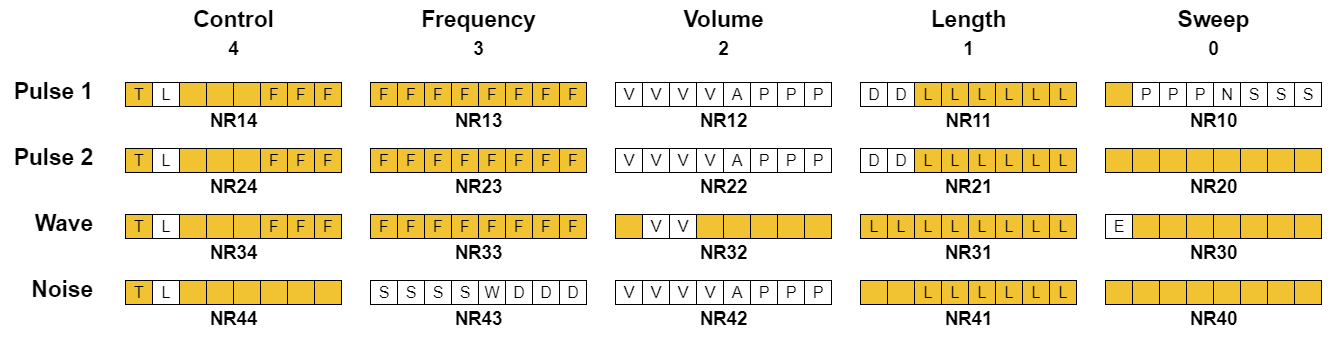
\includegraphics[width=\linewidth]{figures/APU/apu_channel_registers.png}
        \caption{The registers NR10-NR44, addresses \texttt{0xFF10}-\texttt{0xFF23}, for controlling audio channels. Bits coloured in yellow are write only and will always return 1 if read from \cite{AudioHardware}. From \cite{ultimateGBtalkSlides}. Adapted with permission. }
        \label{fig:apu_channel_registers}
    \end{figure}
    
    \begin{table}[h]
        \centering
        \begin{tabular}{|c|c|c|}
            \hline
            \textbf{Label} & \textbf{Name} & \textbf{Functionality} \\
            \hline
            T & Toggle & Turns the channel on or off \\
            \hline
            L (NRx4) & Length enable & \multirow{3}{*}{\shortstack{If the channel should be\\turned off after a short\\period of time}} \\
            & & \\
            & & \\
            \hline
            F & Frequency & \multirow{4}{*}{\shortstack{How long to play\\each audio sample}} \\
            \cline{1-2}
            S, W, D (NR43) & Clock Shift &  \\
            &  LFSR mode & \\
            & Divisor code & \\
            \hline
            V, A, P (Not NR32) & Volume & \multirow{3}{*}{\shortstack{Initial channel volume and how\\it should sweep up or down}} \\
            & Add mode & \\
            & Period & \\
            \hline
            V (NR32) & Volume code & Channel volume \\
            \hline
            D (NR11,NR21) & Duty & Sets pulse length, see Section \ref{sec:theAudioData} \\
            \hline
            L (NRx1) & Length & Time until channel is turned off \\
            \hline
            P, N, S (NR10) & Sweep period & \multirow{3}{*}{\shortstack{Sweeps channel frequency\\up or down to\\create sound effects}} \\
            & Negate & \\
            & Shift & \\
            \hline
            E & DAC power & Turns channel DAC on or off \\
            \hline
        \end{tabular}
        \caption{Description of the labels in Figure \ref{fig:apu_channel_registers}. From \cite{AudioHardware}. Adapted with permission.}
        \label{tab:channel_reg_table}
    \end{table}

% The channels can be turned on or off individually using the bits marked with ``T'' and ``E'' (see registers NRx4 and NR30 in figure \ref{fig:apu_channel_registers}). How long the channel will remain turned on can also be controlled by writing to the bits marked with ``L'', which turns off the channel after a specified length of time. The volume is also adjustable for each channel. For the wave channel there are four volume options ( 00 = 0\%, 01 = 100\%, 10 = 50\%, 11 = 25\%), while for the pulse 1, pulse 2 and noise channel, there are 16 volume options. The volume can also be set to rise or fall over time for these three channels using the bits marked with ``A'' and ``P'' \cite{AudioHardware}.\\
                
% There are some special bits which not all channels have. Notably, the first pulse channel has a sweep register in NR10 (NR30 is not a sweep register despite figure \ref{fig:apu_channel_registers} suggesting it is) which can be used to create sound effects by increasing or decreasing the frequency of the sound while the sound is playing. Both pulse channels also have two bits each, labelled with ``D'' which sets the wave duty mode. The effects of the different modes can be seen in section \ref{sec:theAudioData}. The frequency register of the noise channel looks different from all the other frequency registers, but does similar things but in different ways, see table \ref{tab:frequent_events_apu} for more information \cite{AudioHardware}.

There is also a set of APU master control registers which affects the four audio channels. These can turn the whole APU on or off, indicate what channel is currently playing, and control what side the sound should come from which results in stereo sound. The layout of these registers can be seen in Figure \ref{fig:apu_master_control}. The labels for each bit in Figure \ref{fig:apu_master_control} corresponds to a specific functionality described in Table \ref{tab:control_reg_table}.

\begin{figure}[H]
    \centering
    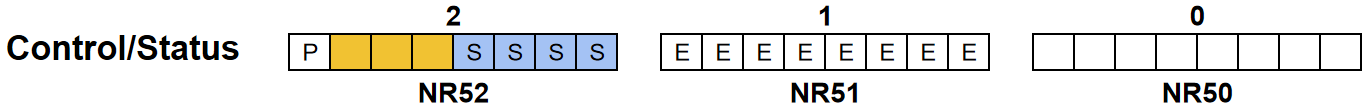
\includegraphics[width=\linewidth]{figures/APU/master_control_apu.png}
    \caption{The registers NR52-NR50, addresses \texttt{0xFF26}-\texttt{0xFF24}, are used for controlling the power and returns the state of all channels. Bits coloured in yellow are write only and will always return 1 if read from. Bits coloured in blue are read only, any data written to this location will be ignored \cite{AudioHardware}.}
    \label{fig:apu_master_control}
\end{figure}

\begin{table}[h]
    \centering
    \begin{tabular}{|c|c|c|}
        \hline
        \textbf{Label} & \textbf{Name} & \textbf{Functionality} \\
        \hline
        P & Power & Enables or disables the entire APU \\
        \hline
        S & State & State of each channel, if 1, the channel is playing \\
        \hline
        L & Left enable & \multirow{2}{*}{\shortstack{Enables or disables left and\\right side for each channel}} \\
        \cline{1-2}
        R & Right enable & \\
        \hline
    \end{tabular}
    \caption{Description of the labels in Figure \ref{fig:apu_master_control}. From \cite{AudioHardware}. Adapted with permission.}
    \label{tab:control_reg_table}
\end{table}

% The registers shown in figure \ref{fig:apu_master_control} displays the registers which controls and shows the power state of all channels. The bit labelled with ``P'' turns on or off the audio hardware and the four bits labelled with ``S'', corresponding to one channel each, is equal to 1 if the channel is playing, and 0 if it does not. The bits labelled with ``E'' also correspond to specific channels and enables or disables the left or right side for each channel. The upper four bits enables or disables the left side, while the lower four bits enables or disables the right side \cite{AudioHardware}.
\newpage
\subsection{Events}
The registers described above trigger events at different frequencies. At what frequency these events should be triggered and exactly what happens at these events is controlled by the registers. Note that all values which are changed with these events are reset when the bit labelled with ``T'' is set \cite{AudioHardware}. The table below summarises the events which occur and at what frequency.
            
\begin{table}[H]
    \centering
    \begin{tabular}{|c|c|c|}
        \hline
        \textbf{Event} & \textbf{Frequency [Hz]} & \textbf{Action} \\
        \hline
        Play sample & \texttt{0x20000}$/(\texttt{0x800} - F)$ & Play next audio sample \\
        \hline
        Play sample (Noise) & \texttt{0x80000}$/ (D * 2 ^ {(S + 1)})$ & Play next audio sample \\
        \hline
        Volume envelope & \texttt{0x40}$/P$ & 
        $V =
        \begin{cases}
            V - 1  & \text{ if A = 0} \\
            V + 1 & \text{ if A = 1}
        \end{cases}$ \\
        \hline
        Length sweep & \texttt{0x100} & Decrease L if length is enabled\\
        \hline
        Frequency sweep (Pulse 1) & \texttt{0x80}$/P$ &
        $F =
        \begin{cases}
            F + F/2^{S}  & \text{ if N = 0} \\
            F - F/2^{S} & \text{ if N = 1}
        \end{cases}$\\
        \hline
    \end{tabular}
    \caption{F, D, S, V, P, L - The value of the bits labelled with ``F'', ``D'', ``S'', ``V'', ``P'', ``L'' respectively, for each channel.}
    \label{tab:frequent_events_apu}
    
\end{table}
      
\subsection{The audio data} \label{sec:theAudioData}
    The pulse wave channels can play a pulse wave with four different waveforms. What waveform to play is specified by the ``duty''-bits, i.e. the bits labelled with ``D'' in Figure \ref{fig:apu_channel_registers}. The resulting waveforms can be seen below in Figure \ref{fig:square_wave_forms}.
        
\begin{figure}[H]
    \centering
    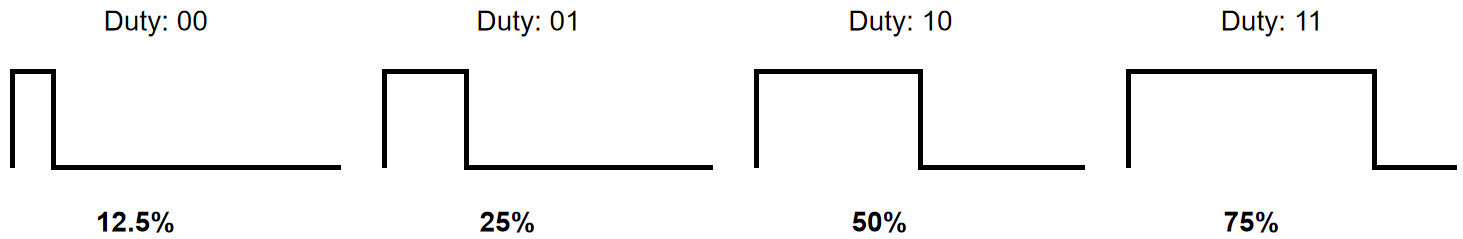
\includegraphics[width=\textwidth]{figures/APU/square_waveforms.png}
    \caption{The four pulse waveforms with their corresponding duties \cite{AudioHardware}. The percentages indicate what amount of the wave is high. Duty ``10'' is   most commonly used.}
    \label{fig:square_wave_forms}
\end{figure}

The waveform of the wave channel can be set to any shape you want by writing to the addresses \texttt{0xFF30} to \texttt{0xFF3F}. Each set of four bits represent one sample which means one waveform consists of 32 samples \cite{AudioHardware}. This approach enables the game developers to create something completely custom made to make their own unique sounds.
\begin{figure}[H]
    \centering
    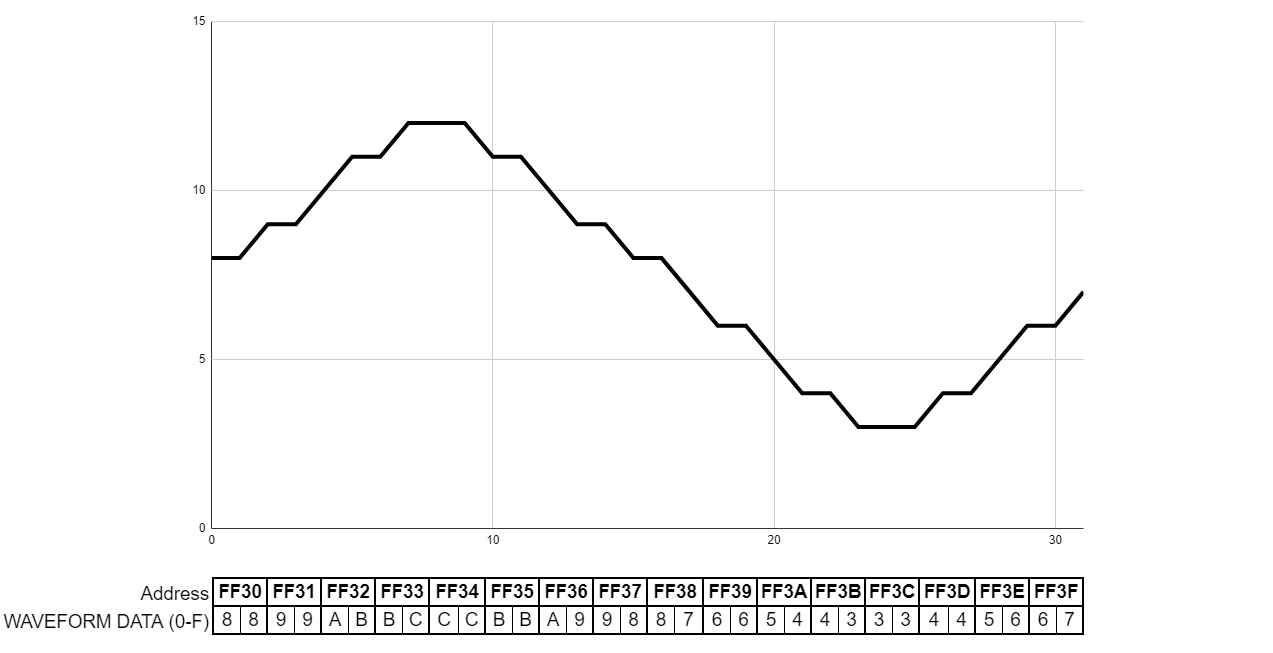
\includegraphics[width=1\textwidth]{figures/APU/apu_custom_waveform.png}
    \caption{A rough representation of how a custom waveform is created through addresses \texttt{0xFF30} to \texttt{0xFF3F}.}
    \label{fig:custom_wave_form}
\end{figure}

The noise channel generates a pseudo-random waveform using a Linear-Feedback Shift Register (LFSR) \cite{apuNoise}. The LFSR is 15 bits long and all bits are set to $1$ in the beginning of the process. Bit 0 in the LFSR determines the output of each sample, if bit 0 is set to one, the output is low, otherwise it is high. To generate a new value of LFSR, the following is calculated where $LFSR(x)$ is the new value, $LFSR(x-1)$ is the old value, $LFSR(x-1)_n$ is the value of bit $n$ in the old value, and $W$ is the value of the bit labelled with ``W'' in Figure \ref{fig:apu_channel_registers} \cite{AudioHardware}.
\begin{equation*}
    LFSR(x) =
    \begin{cases}
        (LFSR(x-1)_0 \oplus LFSR(x-1)_1)*\texttt{0x4000} + LFSR(x-1)/2 & \text{ if W = 0} \\
       (LFSR(x-1)_0 \oplus LFSR(x-1)_1)*\texttt{0x40} + LFSR(x-1)/2 & \text{ if W = 1}
    \end{cases}
\end{equation*}


% METHODS
%\chapter{Method}
\chapter{Tools and methodology}
This section describes the process of planning and implementing an emulator for the Game Boy, the tools used and why they were chosen.% and is followed by the results, presenting what was achieved.
%\section{Tools and methodology}
\section{Programming language}
The language used in the project is C++ \cite{c++}. The language was chosen because it is fast, and supports the bit-level manipulation that is required when emulating hardware.
\section{Graphics and GUI}
For displaying graphics SDL2 \cite{SDL2} and OpenGL \cite{OpenGL} were chosen, mainly due to them being appropriate when developing in C++, as well as the supervisor for this thesis being able to provide a base project already using these libraries which the emulator could be based on. In addition to this the team had some previous experience working with OpenGL.
\\\\
When it came to providing a GUI enabling the user to interact with systems outside of the emulation itself, such as changing/displaying keybinds or loading a game, the library ImGui \cite{ImGui} was used.
\section{Audio}
For generating audio and playing sounds, OpenAL \cite{OpenAL} was used. The choice to implement sound was made partway through the project and the choice then fell on OpenAL as it has a similar design as OpenGL, which the team had already acquired some experience with.


\section{Scrum}
When developing software, it is beneficial to use a flexible work process. When encountering problems or if the scope of the project changes, it should be possible to change direction without requiring the team to rewrite large parts of the project. In order to achieve this flexibility, the working process was formed around the agile development framework Scrum \cite{Scrum}.
\\\\
Whereas traditional Scrum perhaps has not been implemented in this project, the work process has been heavily influenced by Scrum. This is mainly due to the flexibility it allows while developing as well as tracking the work which has been done, and is to be done. This has specifically been done by implementing sprints and using a scrumboard for tracking tasks and progress. Figure \ref{fig:scrumboard} displays what the scrumboard looked like early on in the project.

\begin{figure}[H]
    \centering
    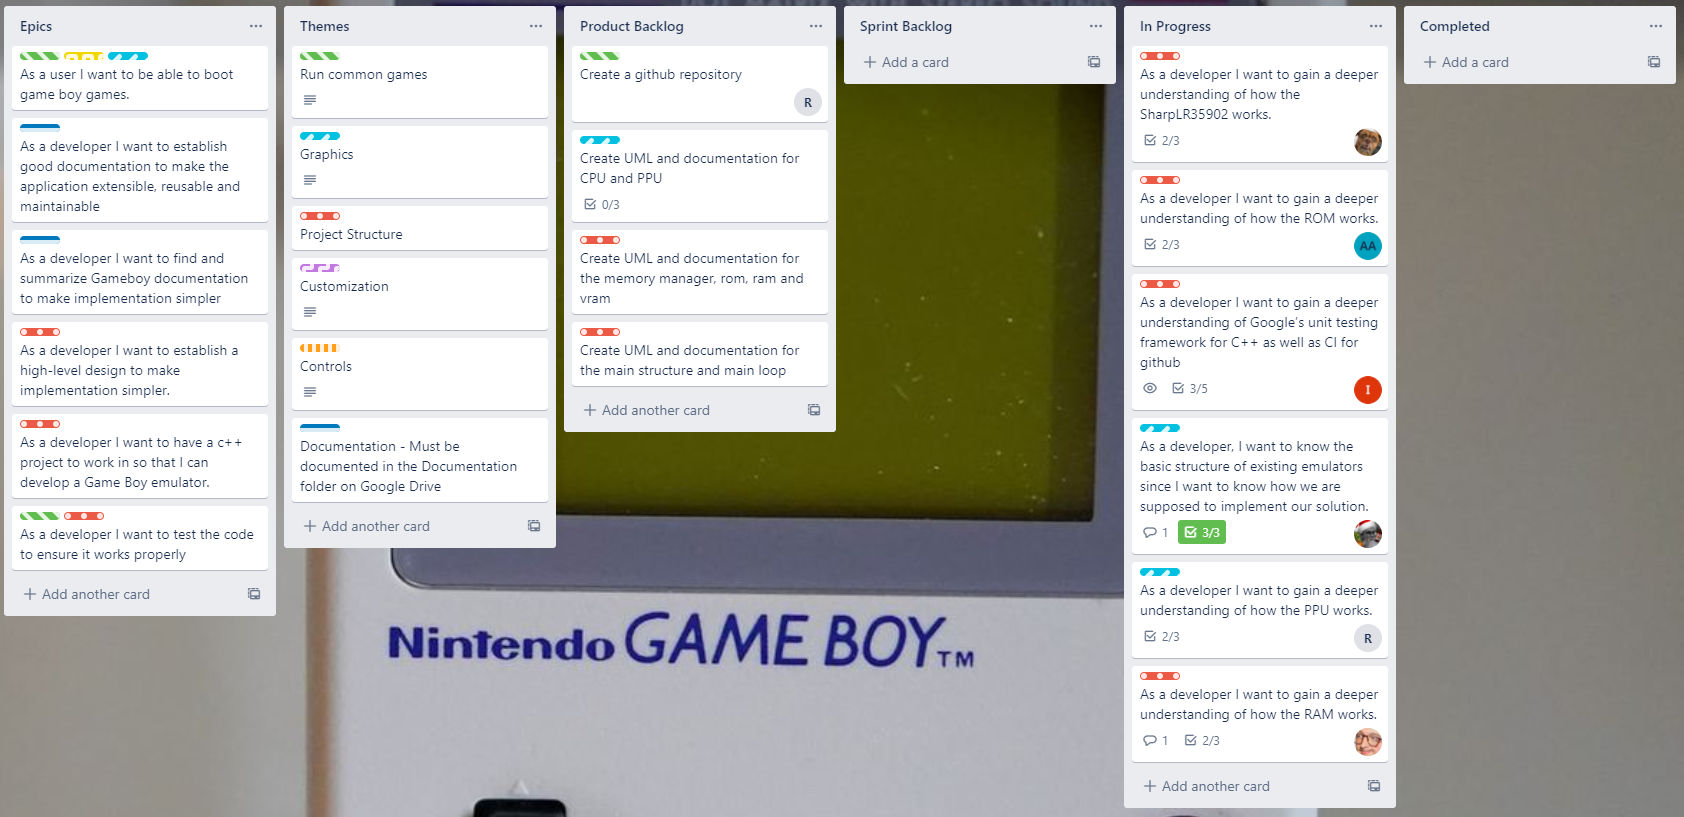
\includegraphics[width=\textwidth]{figures/Scrumboard.PNG}
    \caption{A screenshot of the scrumboard used displaying Epics, Themes, Product Backlog, Sprint Backlog, In Progress and Completed user stories.}
    \label{fig:scrumboard}
\end{figure}

The sprint duration during the period of active development was set to one week as it is usually a suitable duration for a project of this scale. During the other phases of the project, weekly meetings were scheduled resulting in a weekly follow-up during all phases of the project assuming other circumstances such as holidays did not interfere.
\\\\
Additionally, three roles were introduced: A ``Meeting Chairman'', leading each meeting; a ``Secretary'', writing the meeting protocols; and a ``Tester'', making sure all tests pass and responsible for handling pull requests. These roles were created in order to delegate special responsibilities. The roles rotated each sprint, ensuring that none of the group members lagged behind in the development process, whilst also spreading the decision power between all group members. 


%The sprint duration was initially set to one week as it is usually a suitable duration for the size of a project this scale. Three roles were rotated each week; ``Meeting Chairman'' who leads each meeting, ``Secretary'' who writes the meeting protocols and ``Tester'' who makes sure all tests pass and is responsible for handling pull requests. These roles were created in order to delegate special responsibilities. These roles rotate each sprint, ensuring that none of the group members lag behind in the development process, whilst also spreading the decision power between all group members. 

\section{Plan}
The development of this emulator can roughly be split into three phases. The research, implementation and refinement phases, each being different from each other.
\\\\
The main focus of the first phase was researching the Game Boy and finding relevant documentation as this is something which is not provided by Nintendo. By doing this, a basic plan and architecture could be produced. This also included a number of documents summarising information about the Game Boy.
\\\\
Although a rough plan was sketched during this phase, providing both a plan for what to implement and in what order, this was always subject to change as the team had been implementing an agile  workflow allowing for flexibility. Therefore the planning was allowed to be less strict than in other kinds of projects. The planning and documentation produced in this phase still yielded results which could be used as a basis for the second phase. In the end, the development of the emulator followed the Gantt diagram shown in figure \ref{fig:gantt_diagram}.
\\\\
The second phase, implementation, heavily relying on the planning made in the previous phase, followed an agile workflow with sprints being one or sometimes two weeks long. This resulted in a flexible work flow allowing the team to continuously re-assess what to focus on each week while also allowing to document the progress on a weekly basis.
\\\\
The final phase, refinement, allowed for extensive testing, re-factoring and also further development and bug fixing.
\\\\
\newpage
\begin{figure}[H]
    \centering
    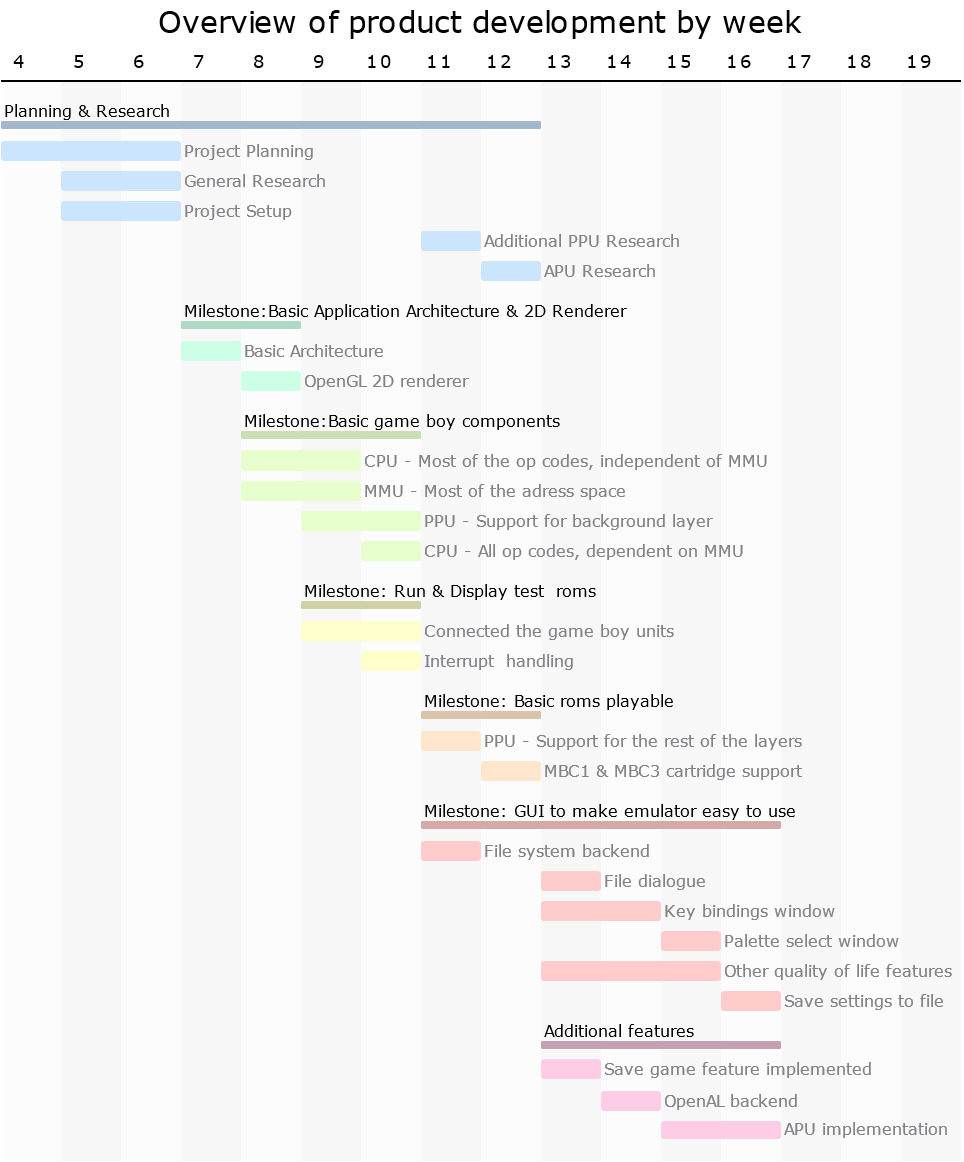
\includegraphics[width =\textwidth]{figures/Gantt diagram.jpg}
    \caption{Gantt diagram over the development of the emulator.}
    \label{fig:gantt_diagram}
\end{figure}
\newpage
\section{Architecture}
%During the first weeks, as research progressed, a basic design was developed where each of the well defined hardware units such as the CPU, PPU and MMU were decided to be separated into one module each. How they would rely on each other and how they would communicate was not 100\% clear due to the fact that not enough research had been done at this stage. It was on the other hand clear that they would need to be separated. 
%Additionally, a sort of Model-View-Controller was chosen as the initial architecture. Although it was never clearly defined exactly how this would be implemented as the knowledge of the chosen graphic libraries were not good enough to be able to assert whether or not this would be possible or necessary.
%Something else which was clear was the fact that there would be a need for an interface where all the separate units of the Game Boy could intersect and work together. Therefore a Game Boy interface was created which one could argue emulates the hardware interface of the actual Game Boy.
During the first weeks, before the development of the actual emulator began, the initial plan was that the emulator would be divided into two larger modules. One module would contain all code related to the actual Game Boy emulation (Game Boy module) while the other would contain code related to the application part of the project such as keyboard input handling, graphics rendering, etc (Application module). For the Game Boy module, a basic design was developed where each of the well defined hardware units such as the CPU and PPU were decided to be further separated into modules. Additionally memory handling was decided to be represented by an aggregate unit resulting in a Memory Management Unit (MMU). For the Application module it was decided that a sort of Model-View-Controller architecture would be used. The final part of this design was an interface where the separate units of the Game Boy could work together and could bridge the gap between the Game Boy module and the Application module.

\begin{figure}[H]
    \centering
    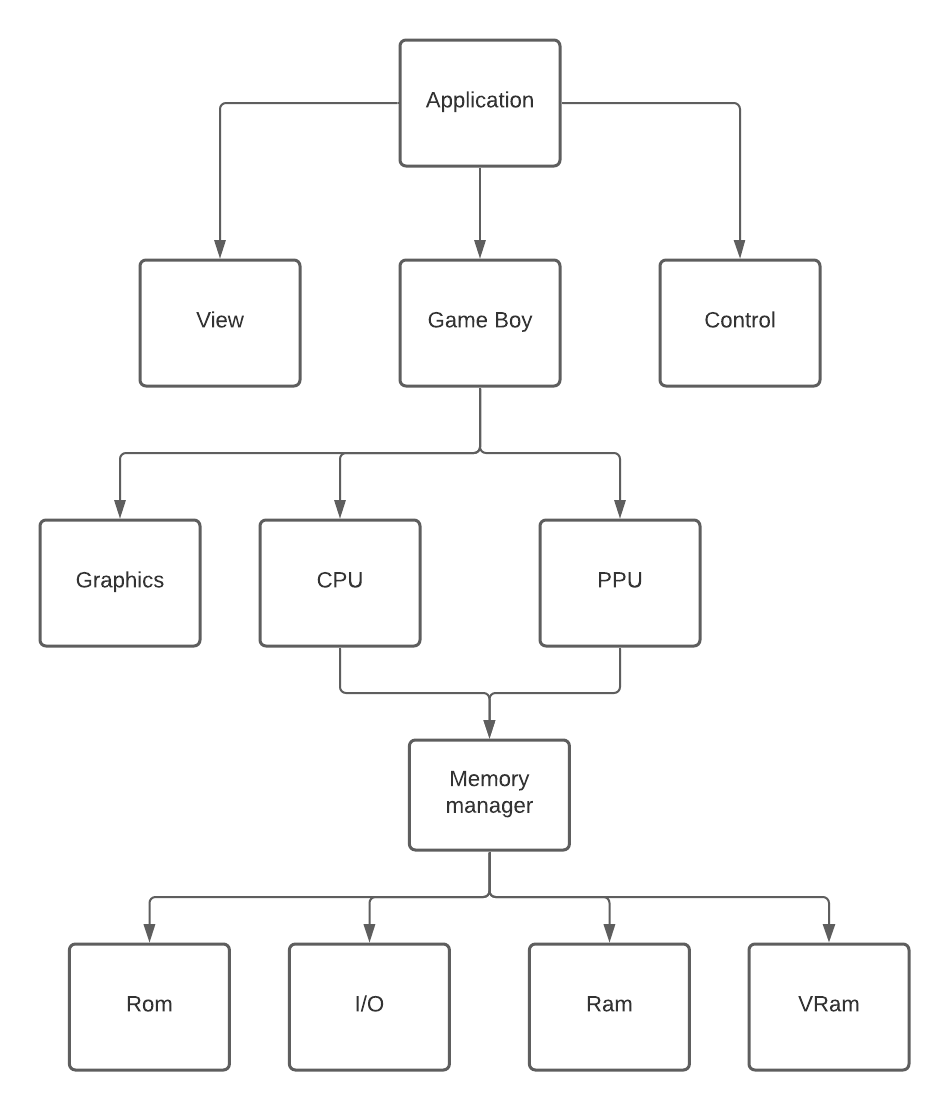
\includegraphics[scale=0.7]{figures/Gameboy Domain model.png}
    \caption{Initial sketch of how different features were to be separated into different modules.}
    \label{fig:initial_domain_model}
\end{figure}

%\section{Development process}
%Something which the original design knowingly did not take into consideration was fact that the different hardware units run in parallel with different clock speeds. This choice was delayed as the research made showed that there were multiple possible solutions to synchronise the different units. Deciding which solution to implement therefore had to be done during development. The chosen solution was to make the CPU return the number of machine cycles after executing an instruction and to then allow the other units to catch up before executing another instruction, see code listing \ref{step}. The shown code snippet displays part of what could be considered the main loop of the emulation. 

\section{Testing}
Unit tests were one of the tools chosen to ensure that the emulator behaves as intended. For this, Google's testing framework Google Test, also known as gtest, was used \cite{gtest}. Google Test was chosen as it supports unit tests for C++ and works well with the Continuous Integration (CI) tool Travis \cite{Travis}.
\\\\
%In addition to the use of unit testing, the Game Boy emulator community has developed several test ROMs with the purpose of being able to ensure that the most critical parts of an emulator are behaving correctly \cite{Blargg}. 
Nintendo have not released any official documentation of the hardware and the exact behaviour of the Game Boy is therefore partly unknown. Due to this, one can not be sure of the accuracy of an emulator, and if certain behaviour is correct or not without comparing the emulator to actual hardware. This of course makes development for the Game Boy more difficult. Fortunately, the Game Boy Wiki provides a table for a set of test ROMs \cite{TestROMsResult} made by the emulator community member Blargg \cite{Blargg}, containing the results of running the ROMs on a number of emulators as well as actual hardware. By comparing these results and the results produced when ran on a specific emulator, one can in some ways confirm whether or not the emulator is behaving correctly. As the community provides a table with the results from Blargg's test ROMs on actual hardware, these were chosen as the first and main test ROMs to be used. In addition to this, some of the tests were deemed more central than others. Specifically the ROMs testing the instruction timing and instruction behaviour.
%In addition to the use of unit testing, the Game Boy emulator community has developed several test ROMs with the purpose of being able to ensure that the most critical parts of the emulator are behaving correctly \cite{Blargg}. Nintendo has not released any official documentation of the hardware and the exact behaviour of the Game Boy is therefore partly unknown. Due to this, one can not be sure of the accuracy of an emulator, and if certain behaviour is correct or not without comparing the emulator to actual hardware. This of course makes development for the Game Boy more difficult.
%\\\\
%The Game Boy Wiki provides a table for a set of test ROMs made by the emulator community member Blargg \cite{Blargg} \cite{TestROMsResult}, containing the results of running the ROMs on a number of emulators as well as actual hardware.
%By comparing these results and the results produced when ran on a specific emulator, one can in some ways confirm whether or not the emulator is behaving correctly. As the community provides a table with the results from Blargg's test ROMs on actual hardware, these were chosen as the first and main test ROMs to be used. In addition to this, some of the tests were deemed more central than others. Specifically the ROMs testing the instruction timing and instruction behaviour.
\\\\
To streamline the testing process, most of the time spent unit testing was done testing the basic operations executed by the CPU, MMU, PPU and in time, the APU. This was done to make sure that the most central parts of the emulator work correctly individually. Once this was done, the test ROMs came into use as these require a working CPU, MMU and PPU as they write the results of the tests directly onto the screen. These produce more extensive results and one might argue that they act as integration tests, testing multiple parts of the code and their interactions. In addition to this, testing was also done by playing a multitude of games, visually looking for bugs and otherwise strange behaviour.
%To be able to test the code, the group chose to use 'Google Testing Framework'. GTF  In addition to unit tests the group decided to use specific test ROMs, to test whether specific instructions and interactions between components are implemented correctly.
%Blargg
%Gtest - Unit testing
%Also playable roms in some way, non proprietary. Compare our emulator vs real game-boy regarding these tests: https://gbdev.gg8.se/wiki/articles/Test_ROMs

% RESULTS
\chapter{Results}

%\section{User Manual}

%\section{Technical Design}
In this section the technical design and implementation of the theory is described.

\section{Architecture and Design}
\label{sec:resultsarchitecture}
The final design of the architecture follows the basics of what was laid out in the initial design with some changes. These changes mostly concern the Application module which was initially planned to follow the Model-View-Controller architecture. The main reason for this is that the chosen GUI library acts as both view and controller. The Application module of the emulator will not be further explored in this section, instead the Game Boy module will be looked at in more detail.
\\\\
The Game Boy module is interacted with through the ``GameBoy''-class which also has the task of synchronising every part of the Game Boy emulation (see below). As mentioned in chapter \ref{chap:Theory}, the different units communicate by reading from and writing to shared address space. This is reflected in the implementation as well as the diagram in figure \ref{fig:dependency_diagram}, which is a dependency diagram of the Game Boy module.

%Since most of the communication between the different Game Boy chips happen through reading from and writing to the shared address space, this is also how it is handled in this emulator. The MMU maintains the shared address space while the PPU, Timer, Joypad, APU and Cartridge classes encapsulates relevant parts of the shared address space. The CPU is not accessible by other Game Boy chips so the MMU does not need to be dependent on it.\\\\\
\newpage
\begin{figure}[H]
    \centering
    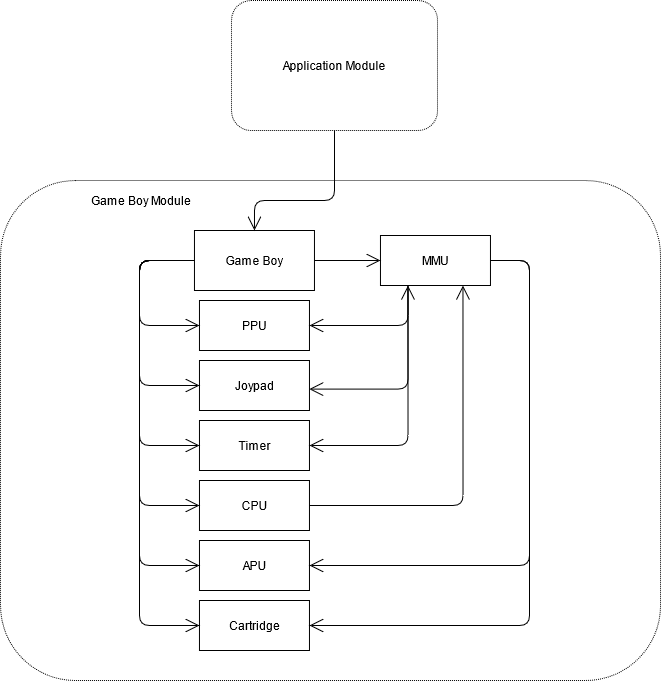
\includegraphics[scale=0.45]{figures/Game Boy Dependencies.png}
    \caption{Dependency diagram over the Game Boy module.}
    \label{fig:dependency_diagram}
\end{figure}
%From the Game Boy class, outside programs can progress the emulation as well as get audio and video data generated by the Game Boy module which can be used to display emulation frames and play audio.\\\\






%The diagram in figure \ref{fig:dependency_diagram} is a dependency diagram over the Game Boy module. This module is interacted with through the Game Boy class which also has the task of synchronising every part of the Game Boy emulation (see below). From the Game Boy class, outside programs can progress the emulation as well as get audio and video data generated by the Game Boy module which can be used to display emulation frames and play audio.\\\\

%Since most of the communication between the different Game Boy chips happens through reading from and writing to the shared address space, this is also how it is handled in this emulator. The MMU maintains the shared address space while the PPU, Timer, Joypad, APU and Cartridge classes encapsulates relevant parts of the shared address space. The CPU is not accessible by other Game Boy chips so the MMU does not need to be dependent on it.\\\\

%\newpage
%\begin{figure}[H]
%    \centering
%    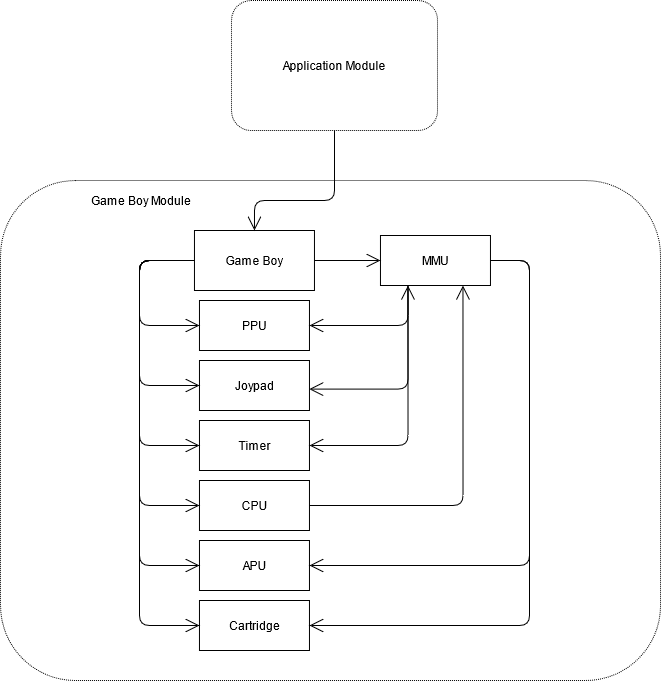
\includegraphics[scale=0.55]{figures/Game Boy Dependencies.png}
%    \caption{Dependency diagram over the Game Boy module.}
%    \label{fig:dependency_diagram}
%\end{figure}

%When the original design was created, a decision regarding how to handle the synchronisation of different units had not been made. Multiple approaches were considered, such as 

Something which the original design knowingly did not take into consideration was the fact that the different hardware units run in parallel with different clock speeds. This choice was delayed as the research made showed that there were multiple possible solutions to synchronise the different units. Deciding which solution to implement therefore had to be done during development. The chosen solution was to make the CPU return the number of machine cycles after executing an instruction and to then allow the other units to catch up before executing another instruction, see code listing \ref{step}. The shown code snippet displays part of what could be considered the main loop of the emulation. 
\begin{lstlisting}[language=C++,
caption = {Code displaying how the CPU executes an instruction and returns the number of machine cycles, whereafter the other units catch up by executing the same number of cycles.},
label = {step}]
void GameBoy::step(IVolumeController *vc){
    ...
    int cycles = cpu->update();
    ppu->update(cycles);
    apu->update(cycles, vc);
    timer->update(cycles);
    cartridge->update(cycles);
    ....
    }
\end{lstlisting}


\section{The Central Processing Unit}
\label{sec:CPUResults}
The implementation of the CPU mainly consists of translating the CPU instructions from assembly to a modern programming language, in this case, C++. The total number of instructions the CPU supports is 500 as mentioned previously, of which many are very similar to each other and all of which are implemented. Due to this, most of the instructions could be generalised into base functions, such as \texttt{add\_8bit} seen in code in listing \ref{addA}. These base operations could in turn handle the variation of the instructions and instead of implementing one function for each operation code, the correct input simply needed to be provided to the correct base instruction given an operation code. There are some exceptions, amongst them the HALT-instruction \cite{HALT-behaviour} which has a very particular behaviour and therefore needed to have a separate implementation.
\\\\
\begin{lstlisting}[language=C++,
caption = {Code displaying a generalised method used, in this case an addition function which allows for addition between register A and all other registers, both with and without the use of the carry bit.},
label = {addA}]
void CPU::addA(uint8_t value, bool withCarry) {
    add_8bit(A, value, withCarry);
}

void CPU::add_8bit(uint8_t &a, uint8_t b, bool withCarry) {
    auto CFlag = withCarry ? F.c : 0;
    setCFlag(a, b + CFlag, false);
    setHFlag(a, b, false, CFlag);
    a += b + CFlag;
    //Note that all 'false' parameters specify that subtraction is not used, which in turn affects how and which flags are set.
    setZNFlags(a, false);
}
\end{lstlisting}

\subsection{Interrupts}
As previously stated, the CPU has five types of interrupts. Of these five only the ``Serial interrupt'' is not implemented, which there never was any intention of implementing as mentioned in section \ref{sec:Delimitations}. All the implemented interrupts are in some ways central in having a working CPU as these allow for other units to request the CPU to perform specific tasks when needed.
\\\\
\subsection{Testing}
Mainly, three tests were used for checking the accuracy of the CPU. These check the correctness of the instructions \cite{Blargg}, their timings and the interrupt timing respectively. The tests regarding the CPU-instructions, \texttt{cpu\_instrs} and \texttt{instr\_timing}, pass on both the real hardware \cite{TestROMsResult} and the emulator see figure \ref{fig:cputests}. 
\\The \texttt{interrupt\_time} test, however, does not pass despite being implemented and performing as expected. It most likely fails due to the implementation of the synchronisation of the different units. This is further discussed in section \ref{sec:CPUDiscussion}. 

\begin{figure}[H]
\centering
\begin{subfigure}{.5\textwidth}
  \centering
  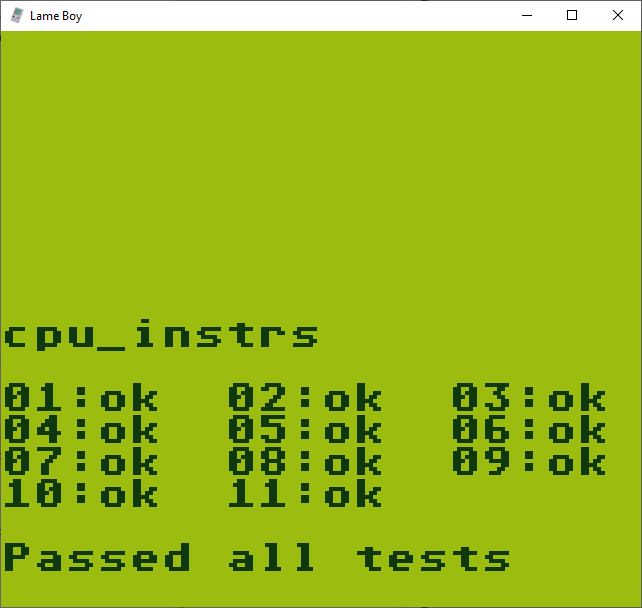
\includegraphics[width=0.9\linewidth]{figures/cpu_instrs_passed.PNG}
  %\caption{Figure displaying the emulator passing Blargg's test checking the correctness of the CPU instructions.}
  %\label{fig:cpu_instrs}
\end{subfigure}%
\begin{subfigure}{.5\textwidth}
  \centering
  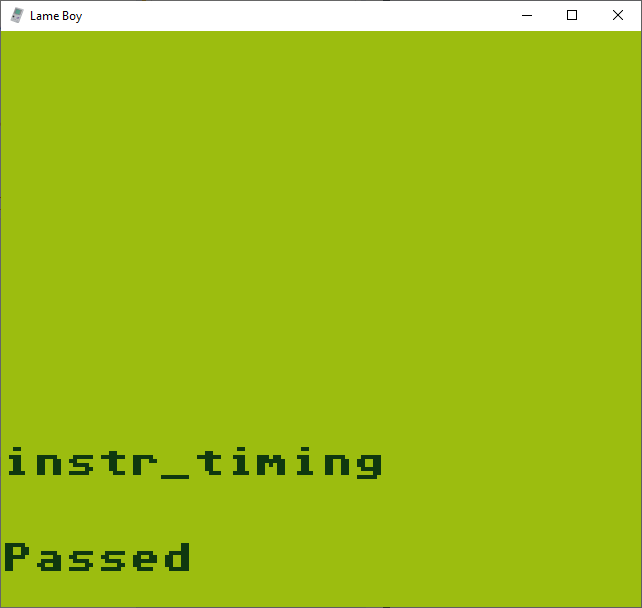
\includegraphics[width=0.9\linewidth]{figures/instr_timing_passed.PNG}
 % \caption{Figure displaying the emulator passing Blargg's test checking the correctness of the CPU timing.}
  %\label{fig:instr_timing}
\end{subfigure}
\caption{Displaying the emulator results from  Blargg's test ROMs checking the correctness of the CPU instructions and CPU timing respectively.}
\label{fig:cputests}
\end{figure}   

%There are a number of additional test ROMs, amongst them mooneye-gb \cite{Gekkio-Mooneye}. Many of these have not been run on the emulator as of yet, and no results from these can therefore be presented. However, as the CPU is passing the most central tests, the ones regarding instruction correctness and timing; which affect not only the CPU but all hardware units, further work regarding improvement of the accuracy of the CPU was put on hold.

\section{The Memory Managing Unit}
The Game Boy uses memory mapped I/O which means that almost all communication can be done through reading and writing to the different addresses. Therefore the main purpose of the MMU is to provide functionality which supports reading memory and writing to memory. 
%Because the Game Boy uses memory mapped I/O almost all communication can be done through reading and writing to the different addresses.
%Therefore the main purpose of the MMU is to have a read and a write function which in turn calls a specific device's read and write function.
%The read function is supposed to return the value on the given address. The write function is supposed to write the given value to the given address.
\\\\
To separate code and improve the possibility for parallel development all the different devices are separated into their own classes: PPU, APU, Cartridge, Joypad and Timer, each having their own read and write functions. 
The memory addresses used by the device (mostly control registers) are also maintained in the devices' class. 
The other memory areas which are not part of a device are located directly in the MMU class. Examples of such memory are: boot ROM, VRAM, WRAM, OAM, and HRAM.

\subsection{Timer}

The timer is implemented as a device with read and write functions. 
Reading and writing to the timer's four registers is implemented to behave as described in the section \ref{sec:MMUTheory}.  
To make the timer update at the same pace as the CPU (and the system as a whole) it has an update function. 
The update function allows the timer to catch up to the system based on the number of cycles required for the last CPU instruction executed, see section \ref{sec:resultsarchitecture}.
Because of the timer not being updated continuously it is not always accurate. On original hardware the counter would increase during the execution of a CPU instruction and could therefore change between the start of the execution and the actual read from the counter register.


% Updated based on the cpu instruction.
% Not completely accurate, (skipping counts).


\subsection{Cartridges and Memory Bank Controllers}
Due to the fact that there are a number of different game cartridges, all supporting different hardware, such as different MBCs, RTC, ROM and XRAM sizes, a modular approach was taken. 
This was possible as although the cartridges may have different hardware they operate in a similar manner, therefore an MBC interface class was made.
This enables different behaviour when reading or writing to the cartridge's addresses depending on the used MBC. The MBC interface also uses an update function to allow the possibility of an RTC to update at the same pace as the rest of the system. This function updates the RTC according to the specified number of clock cycles, see section \ref{sec:resultsarchitecture}. For MBCs without an RTC this function does not do anything. This way multiple MBC classes can be implemented to easily expand the support for different MBCs. The most common MBCs are MBC1 and MBC3, which are also the ones which have been implemented.
%The MBCs that are used in most common games are the MBC1 and MBC3 which is the ones that have been implemented.
\\\\
The information about hardware used in each game is stored in the game ROM file.
When loading the ROM file into memory the MBC type, ROM size and XRAM size can be obtained and initialised accordingly. 
Another feature for games with XRAM supported with a battery is the ability to save data between different sessions.
A common way to support this in emulators, this one included, is to create a separate file to save the current contents of the XRAM to. Meaning that when loading a ROM file, the emulator also looks for an XRAM-file, which if found is also loaded and initialised, providing a way to use a games' built in save functionality.

\subsection{Testing}
Testing of the implemented MBCs has been done using test ROMs that test different features of the MBC such as ROM and XRAM bank switching as well as the RTC. The MBC tests used are Gekkio's mooneye-gb tests \cite{Gekkio-Mooneye} and aaaaaa123456789's rtc3test \cite{mbc3test}, which the emulator pass.
\\\\
Testing the timer was done with some test ROMs from Gekkio's mooneye-gb tests \cite{Gekkio-Mooneye}. Most of them do not pass, most likely due to the inaccuracies caused by the update function. Although, its basic counting capability has been tested through games that for example use the counter to produce randomness. Without the counter the supposed randomness did not produce different outcomes, but with the timer implemented the outcome seemed more random.

% Passing a couple of tests but fail most of them. Probable because inaccuracy in updates. Works for randomisation in Tetris.

\section{The Pixel Processing Unit}
The PPU class aims to replicate the functionality of the PPU in the Game Boy. In this section, the term ``PPU'' will refer to the PPU class and the term ``original PPU'' will refer to the Game Boy's PPU.\\
\\
The PPU contains the same registers as the original PPU and implements read and write methods that the CPU uses to communicate with the PPU.

\subsection{Timing}
As mentioned in \ref{sec:resultsarchitecture}, the PPU is controlled by a different clock than the CPU and need to be kept in sync. To solve this problem, the PPU is updated every time a CPU instruction is executed. By providing the number of cycles the CPU instruction used to the update-method of the PPU, it is possible to determine how much time has passed since it last switched mode and thereby decide whether the PPU should switch mode or not. For simplicity, the PPU also does all the real ``work'' of a mode whenever it switches from that mode.

\subsection{Basic operation}
The basic operation of the PPU is described by the update-method. Firstly, the PPU adds the number of cycles elapsed since the last CPU instruction was executed to the number of accumulated cycles since the PPU last switched modes, as seen in \ref{sec:resultsarchitecture}. It then checks whether or not it should switch mode. This calculation is based on the durations in table \ref{tab:PPU_mode_durations}; That is, the draw mode has been set to take the fewest amount of cycles that it can possibly take in the real Game Boy and the h-blank has been set to take as much time as is possible. When this is done, the PPU checks whether a STAT-interrupt should be requested and if so requests one.
\begin{table}[H]
    \centering
\begin{tabular}{l|l}
    \textbf{Mode} & \textbf{Cycles} \\
    \hline
    H-blank & 51\\
    V-blank & 144\\
    OAM-search & 20\\
    Drawing & 43
\end{tabular}
\\\
    \caption{The durations of the PPU's modes}
    \label{tab:PPU_mode_durations}
\end{table}
What happens when the PPU changes mode depends on which mode it was just in. This is very similar to the basic operation described in section \ref{sec:PPU_Modes} but there are a few differences, the main ones being that the image is rendered one line at a time and that the CPU has free access to VRAM and OAM at all times. The operation during the various modes is described below.\\
\\
\textbf{H-blank}\\
When leaving an h-blank, the PPU moves on to the next scanline. The LY register is therefore increased by one. If all lines have been drawn, the PPU moves to v-blank mode and a v-blank-interrupt is requested. If not, the PPU goes into OAM-search mode.\\
\\
\textbf{V-blank}\\
The v-blank in the emulator is treated as ten blank scanlines, since the v-blank in the Game Boy lasts for ten lines. Therefore, the LY register is increased by one every time the PPU is done with a blank scanline. If all ten blank scanlines have passed, LY is reset to 0 and the PPU goes into OAM-search.\\
\\
\textbf{OAM-search}\\
When leaving OAM-search the PPU prepares the sprites to be drawn on the current line by adding the ones that intersect with the line to a priority queue. This ensures that when retrieving the sprites from the queue, the ones with highest priority will be drawn above those with lower priority. The PPU then goes into drawing mode.\\
\\
\textbf{Drawing}\\
When leaving the drawing mode, the PPU processes the next line by calling the \texttt{processNextLine} method and then goes into h-blank mode. The drawing process is described in detail in section \ref{sec:result-drawing}.

\subsection{Drawing}
\label{sec:result-drawing}
Unlike the original PPU, which draws pixels directly to the LCD, the PPU instead inserts pixels into a frame buffer. Scanlines are drawn one at a time, but the layers background, window and sprites are drawn in that order on top of each other, depending on which of these layers are enabled in the LCDC register.\\
\\
\textbf{Background}\\
For a given scanline, for each x-coordinate, the PPU determines the tile corresponding to the coordinate, then which pixel of the tile should be drawn and lastly which colour it should have. The colour is written to the frame buffer and the colour index is saved in an array containing the background and window colour indexes for the current line. This array is later used for determining sprite priority over the background.\\
\\
\textbf{Window}\\
For a given scanline, the PPU first determines whether the window covers this scanline. If it does, the window pixels are written to the frame buffer in a similar manner to how the background is written. Any background pixels covered by the window are overwritten.\\
\\
\textbf{Sprites}\\
For each sprite found during OAM search, in order of ascending priority, the PPU draws the correct tile. If a pixel is transparent, the PPU simply moves on to the next pixel. If a sprite is to be drawn below the background, the array containing background and window indexes is used to determine the correct pixel.

\subsection{DMA transfer}
\label{sec:DMA_transfer_result}
The DMA transfer in the emulator functions exactly the same as the one in the original Game Boy described in \ref{sec:DMA_transfer}, with the exception that the process does not consume any cycles. That is to say, the entire DMA transfer takes place before the CPU is allowed to execute its next instruction.

\subsection{Testing}
The correctness of this module was mainly tested through visual observations. Unit tests were written to ensure correct behaviour of the PPU with various settings turned on or off in the LCDC register. Examples are correct scrolling, using different tile maps and tile sets and ensuring that the window covers the background.\\
\\
Testing was also done by running game ROMs and comparing them to gameplay on the original Game Boy as well as other emulators.

\section{The Audio Processing Unit}

%Before integrating the OpenAL library with the emulator code base, a separate minimal project was created which was only used to play sound and to learn how the OpenAL library worked. The relevant code was then copied into the emulator project.
% \\\\
Since the APU is composed of multiple audio channels, features and controls, it was decided that the first square wave channel, without the frequency sweep functionality, should be implemented first. After getting this first audio channel working, the other audio channels were implemented iteratively along more complicated features such as volume and frequency sweep.

\subsection{The Audio Controller}
An audio controller class was created whose responsibility is to play sound using the OpenAL library. Due to how the OpenAL interface works, this class cannot play one sample at a time, but instead relies on being fed an array of samples which should be played at a specific frequency for a specific amount of time. In order to play a sound for any length of time, only the samples of one waveform is provided which is then looped until stopped. Since the square wave and programmable wave channels already have a predefined waveform, this was trivial to implement. The noise channel does not and therefore was more difficult.
\\\\
Since the waveform of the noise channel is pseudo-random, OpenAL must be provided with more than one waveform. Thankfully, it was discovered from testing that the $LFSR(x)$ function which is used to generate pseudo-random noise, specified in section \ref{sec:theAudioData}, loops at $x = $ 0x7F when $W = 1$ and at $x = $ 0x7FFF when $W = 0$. This means only two arrays need to be generated, one of size 0x7F and one of size 0x7FFF, which can be provided to OpenAL while also instructing OpenAL to loop the sound, resulting in an infinite noise sound.
\\\\
Due to the interface of OpenAL, the frequency of a sound cannot be changed while playing. Changing the frequency therefore requires the sound to be stopped before being played again at the new frequency. The effects of this are noticeable when a game uses the frequency sweep register since there are fast consecutive switches between frequencies. Instead of sounding like dragging your finger across a piano, it sounds like dragging your thumb across the teeth of a comb.

\subsection{Testing}
When testing the APU, games were played on the emulator and the sound generated was compared with sound from videos on YouTube where the same game was played. Aspects such as what tone was played, at what moment, for how long and at what volume was observed when testing each register of each audio channel. This resulted in the APU to be an approximation of the real APU where small technical details was ignored.
\\\\
The more advanced features such as the frequency and volume sweep were difficult to replicate accurately. To test these features, the ``Sound Test (PD) [a1]'' \cite{SountTestPD} ROM was run which allows the user to set specific parameters in the APU registers and play the specific sound channels. This ROM was also run on existing emulators, like the Visual Boy Advanced \cite{visualBoyAdvanced}, in order to compare the results.
\\\\
Similarly to when testing the CPU, Blargg's test ROMs \cite{Blargg} were also used to test the APU. In particular, the \texttt{dmg\_sound} test ROM was run in order to test the sound of the emulator. However, since many of the small technical details of the APU were ignored, not many of the tests passed, as seen in figure \ref{fig:blargg_dmg_sound}.

\begin{figure}[H]
    \centering
    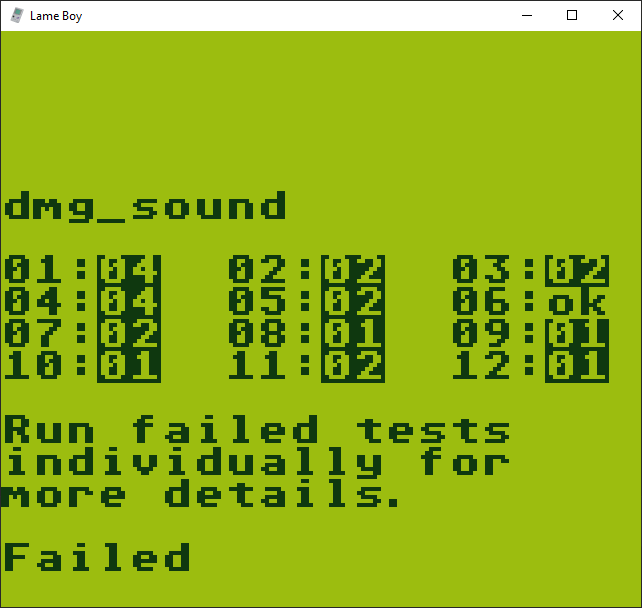
\includegraphics[width=\textwidth/2]{figures/APU/blargg_dmg_sound.PNG}
    \caption{Results of running the \texttt{dmg\_sound} test ROM from Blargg's test ROMs \cite{Blargg}.}
    \label{fig:blargg_dmg_sound}
\end{figure}

\section{The Game Boy}
After having developed multiple microcontrollers, they were combined into a complete system as described in section \ref{sec:resultsarchitecture}. This system is the public interface of the hardware units and could be considered the actual emulation of the Game Boy. In combining these microcontrollers an emulator is created which in its current state can run multiple games without issue and in many ways provide an authentic experience. There are however games containing bugs, both mechanical and visual, and demonstrating irregularities such as crashes or other unwanted behaviour.
\\\\
In code, this is represented by a separate ``GameBoy''-class which combines all of the developed microcontrollers. It is through this the emulation is run and through this, all information is funnelled to external libraries such as OpenGL, ImGui and OpenAL.

\begin{figure}[H]
    \centering
    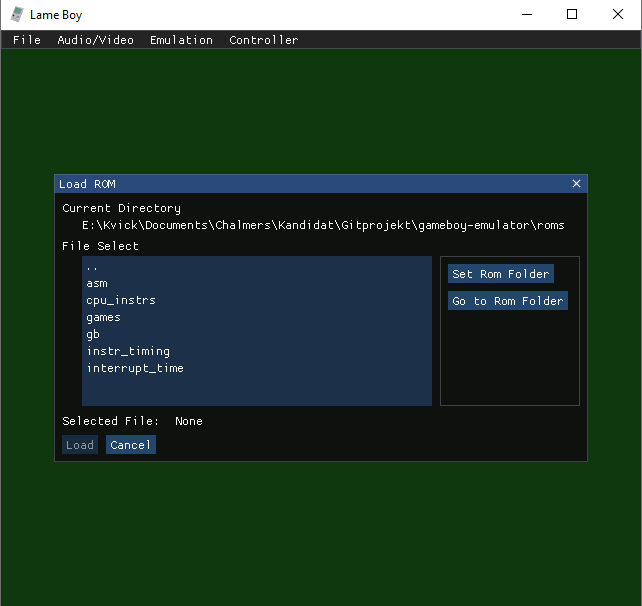
\includegraphics[width=0.7\textwidth]{figures/emulator.png}
    \caption{A screenshot of the emulator when loading ROMs.}
    \label{fig:emulator_picture}
\end{figure}

% Discussion
\chapter{Discussion}
This chapter will discuss the results of the project. If there were any specific problems or choices in implementation which was made, and why.

\section{Hardware}
There is very little, if any, official documentation available regarding the specifics of the hardware used in the Game Boy. While this complicates emulator development, there are members of the community who have dedicated a lot of resources into providing accurate documentation on the hardware. Among these are two of the co-authors of PanDocs \cite{pandocs}, Gekkio \cite{Gekkio.fi} and Antonio Niño Díaz \cite{AntonioND}. Both of which are also authors of their own very detailed documentations of the Game Boy, the ``Game Boy: Complete Technical Reference'' \cite{CompleteTechnicalReference} and ``The Cycle-Accurate Game Boy Docs'' \cite{TCAGBD} respectively. These two documents are based on tests written and ran on multiple units of the real hardware to ensure that they are testing correct behaviour, and thereby providing a way to reverse engineer the hardware. These sources, or sources similar to these, have therefore been central in the development of this emulator.

\subsection{CPU}
\label{sec:CPUDiscussion}
While implementing the CPU, a problem regarding the number of machine cycles an operation required was encountered. The problem was that the source used for the operation codes \cite{OpCodes}, which displays flags affected, number of bytes used and number of machine cycles, was not the same as used in Blargg's test ROMs \cite{Blargg}. As the test ROMs have been run on the real hardware and passed the tests, the team considered the test ROMs to be using the correct amount of cycles \cite{TestROMsResult}. A process similar to what Gekkio and Díaz applies in their testing.
\\\\
Looking at Blargg's test suite regarding the CPU tests, one might note that the emulator does in fact not pass all tests. Among the tests which it does not pass are the \texttt{interrupt\_time}, \texttt{mem\_timing} and \texttt{mem\_timing-2} \cite{Blargg}. As mentioned in section \ref{sec:resultsarchitecture}, the different units need to be synchronised and act in accordance with each other. There are indications that the reason for the tests failing is that it is possible for the CPU to execute too many machine cycles before allowing the other units to catch up or interrupts to intercept. Meaning that the current implementation of the CPU does not allow for timer updates mid-instruction. In hindsight, it is possible this could have been avoided by allowing for this to happen between the MMU reading or writing while the CPU is executing an instruction.
\\

\begin{comment}


\begin{lstlisting}[language=C++,
caption = {Code displaying how the CPU executes an instruction and returns the number of machine cycles, whereafter the other units catch up by executing the same number of cycles.},
label = {step}]


void GameBoy::step(IVolumeController *vc){
    ...
    int cycles = this->cpu->update();
    ppu->update(cycles);
    apu->update(cycles, vc);
    timer->update(cycles);
    cartridge->update(cycles);
    ....
    }
\end{lstlisting}
\end{comment}

\subsection{MMU}
Early in the development all memory and registers were located directly in the MMU class. 
When first implementing the PPU it always needed to ``fetch'' the registers it needed from the MMU to continue to do its job.
This made it clear that it would be better to make the different device classes keep their own registers.
With this change it was necessary but also natural to make use of individual read and write functions for each device, which in turn would be called from the main read/write function located in the MMU class.
\\\\
In the memory map, seen in figure \ref{fig:memory-map}, there are some areas that are empty.
Although Nintendo says use of these areas are prohibited they still have a specific behaviour confirmed on all official hardware \cite{pandocsechoram}.
The seemingly empty range \texttt{0xE000}-\texttt{0xFDFF} is by the community called ``Echo RAM'' and is on the original hardware mapped to the actual RAM addresses.
For example, writing a value to address \texttt{0xE001} would have the same effect as writing to the address \texttt{0xA001}. Same goes with reading values.
We have chosen to not implement this behaviour mainly just because it is prohibited by Nintendo and is expected to be unused in licensed games. 
Additionally, this behaviour does not add any functionality that cannot be achieved by other means.
Furthermore, if it is used in unlicensed games it is easily implemented down the line.  
\\\\
The choice to only implement two different MBCs was made because the most popular games make use of these MBCs. 
Implementing more MBCs would yield less return for the time spent and time was therefore put into other areas that felt more important. Also, as previously mentioned, a modular approach was taken when implementing MBCs, making it easy to implement in the future if wanted.
\\\\
The access limitation of different memory areas has not been implemented, as this is expected to be respected by game developers. For example, during a DMA-transfer the CPU, on the original hardware, is limited to only access HRAM during that period.

\subsection{PPU}
As mentioned both in sections \ref{sec:CPUDiscussion} and \ref{sec:PPU}, the choice to synchronise the different units with the CPU was done by supplying the other units with how many machine cycles the CPU executes from completing one instruction. The biggest limitation of doing the primary work this way regarding the PPU is that the emulator does not support writing to PPU hardware registers mid-scanline. This results in graphical glitches in a few games, but is not a problem for a vast majority of games. However, the emulator supports writing to hardware registers between scanlines, enabling visual effects such as the one shown in figure \ref{fig:flappyboy}:


\begin{figure}[H]
\centering
\begin{subfigure}{.5\textwidth}
  \centering
  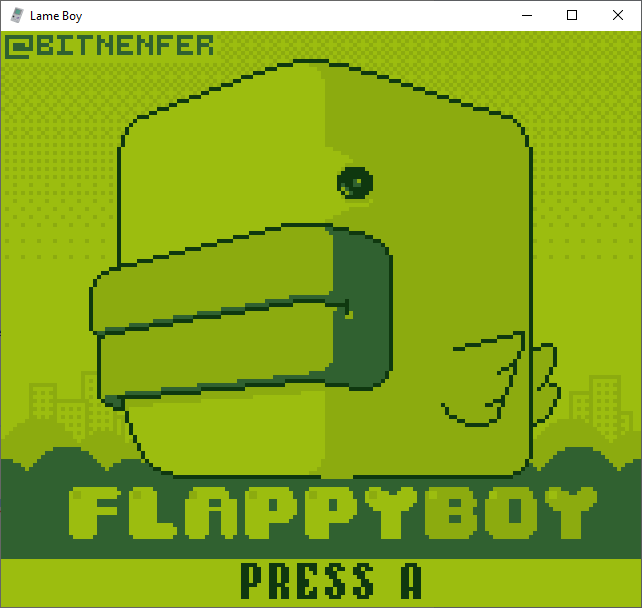
\includegraphics[width=0.9\linewidth]{figures/PPU/Flappyboy_normal.PNG}
  %\caption{Figure displaying the emulator passing Blargg's test checking the correctness of the CPU instructions.}
  %\label{fig:cpu_instrs}
\end{subfigure}%
\begin{subfigure}{.5\textwidth}
  \centering
  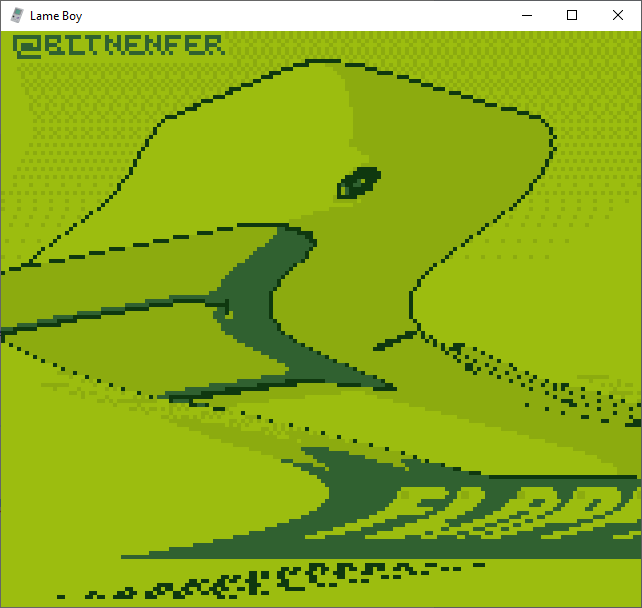
\includegraphics[width=0.9\linewidth]{figures/PPU/Flappyboy_distorted.PNG}
 % \caption{Figure displaying the emulator passing Blargg's test checking the correctness of the CPU timing.}
  %\label{fig:instr_timing}
\end{subfigure}
\caption{The starting screen of the game Flappyboy. From left to right, its original form and its distorted form achieved by writing to the SCX and SCY registers between scanlines. From \cite{FlappyBoy}. Screenshot by authors, used with permission.}
\label{fig:flappyboy}
\end{figure}   

The decision to render the image scanline by scanline was made as it supported the aforementioned wobble effect and other visual effects, while still being achievable within the given time frame. To support writing to hardware registers mid-scanline would require a much more accurate simulation of the original PPU and was not feasible in the allotted time.\\
\\
Another difference between the emulator and the original PPU is that the emulator does not limit the CPU's access to VRAM and OAM. This could lead to bugs in games where the developers have not ensured that the CPU has access to VRAM or OAM before reading or writing to these memory areas.\\
\\
All in all, graphical glitches are few and far in between and the PPU must therefore be considered correctly implemented within the scope of the project.

\subsection{APU}
Implementing sound was initially considered out of scope, as it was deemed too complex and would take too much time to implement. Therefore any progress made in this regard is seen as exceeding the initial expectations. As the development of the other parts progressed faster than expected, there was time to spare which allowed the group to implement the APU.
\\\\
%Creating a small separate project, only for checking out the the OpenAL library what helpful since it allowed us to only keep the code we wanted. It also allowed us to check that the library worked for all group members which used different platforms.
Only implementing one channel at a time was a good choice as once the first channel had been implemented, it was easy to implement more. The biggest difference between  the sound channels was how the audio was generated. Thankfully they could be implemented similarly without changing much but the audio data provided to the OpenAL API.
\\\\
However, the devil is in the details, and for the APU there are a lot of them. There have been several issues where sound continues to play when it should have been muted, sound beginning to play from nowhere when it is not suppose to etc. Most of these issues have been resolved, but there are still existing issues with some games where the audio does not play at all.
\\\\
The room for improvement is also apparent in the results of running Blargg's \texttt{dmg\_sound} \cite{Blargg} test ROM which, as seen in figure \ref{fig:blargg_dmg_sound}. Almost all tests fail due to these small details not being implemented. But as said before, we are glad to have been able of making some games work well, and getting any sound at all has exceeded our expectations of the project.

\section{Planning}% and Scrum?}
The initial plan was created to simplify the organisation of the project and to early have an overview of the project. The plan was followed quite strictly during the first few weeks until the team entered the implementation phase where an agile workflow was implemented. This turned out well as being able to re-assess and re-prioritise what needed to be done at a given stage of development is very important for many reasons. One of the reasons was that the team during the period of developing this emulator also had other commitments and deadlines. Additionally, the development of some parts of the emulator required more time than expected, and some less. %For example, the initial plan supposed that a basic CPU, PPU and MMU should be working during week 7, allowing a boot ROM to be run. For reference, this is about two weeks into development. It was not possible to run a boot ROM until mid week 9, which is another two weeks into development. 
\\\\
\section{Accuracy}
One thing to always consider when discussing the development of emulators is the accuracy of the emulation, and specifically how accurate the emulator aims to be. Some developers choose to try to emulate the exact behaviour of the hardware, including what today could be considered bugs, flaws or mistakes. Others seize the opportunity and corrects some behaviour of the emulator which they deem incorrect or faulty.

\subsection{Compromises}

Given the scope and the time spent on this project, our emulator had to make compromises between accuracy and progress. Assuming the aim would have been to be as accurate as possible, a lot more research would have had to been done, and implementation could and would have had to be planned more carefully. On the other hand, many of the systems implemented are implemented with the intention of making it extensible, and easy to further develop and add to the emulator.
\\\\
One of the compromises which was made was considering the choice of further developing the CPU, making it more accurate and passing more test ROMs, like Blargg's interrupt timing test \cite{Blargg}, or attempting to implement sound. Adding sound to the emulator would increase the overall impression and feeling of the emulator, while there is no guarantee that making the CPU more accurate would increase the user experience in any way. One might even argue that implementing additional features such as saves, a functional GUI and other quality of life features yields a better overall impression than improving the accuracy of the emulation. Therefore the choice fell on trying to implement sound and other, smaller features.

\subsection{Vital and auxiliary components}

Some components of the Game Boy are more important than others, which means these have to be more accurately emulated than auxiliary components. The most vital component to be emulated accurately was the CPU since it is the central component of both the Game Boy and the emulator. Any bugs caused by the CPU may result in obscure behaviours which can be close to impossible to debug. Getting Blargg's \texttt{cpu\_instrs} and \texttt{instr\_timing} \cite{Blargg} test ROMs working was therefore highly prioritised in order to validate the accuracy of the CPU and avoid any of these potential bugs.
\\\\
The APU, which on the other hand could be considered an auxiliary component, was not given the same attention in regards to accuracy as the consequences of having a defective APU is not as severe. The worst thing that could happen with the APU is the absence, or constant presence, of sound, but all other parts of the emulator should still work as intended. This is because, in contrast to the CPU, no other component strictly relies on the APU to perform its function accurately. The results of this approach to accuracy is visible in figure \ref{fig:blargg_dmg_sound} which shows only test \texttt{06} passing when running Blargg's \texttt{dmg\_sound} \cite{Blargg} APU test ROM.


\section{Ethics}
As mentioned in section \ref{sec:introEthics} the emulation of a proprietary product comes with both ethical and legal complications, some of which are discussed in this section.
\label{sec:Ethics}
\subsection{Legality of emulators vs. ROMs}
Most digital copyrighted material have some sort of controversy around them. Gaming consoles and their respective emulators are no different. Like most subjects touching on potential piracy and copyright infringement, there is a huge grey zone whether or not something is legal or illegal, and subsequently if something is right or wrong. 

\subsection{The emulator}
The creation of a game emulator is generally not illegal as long as no proprietary code is used \cite{emulatorLegal}. This is mainly because the emulator itself does not necessarily have to contain any proprietary code to replicate the original console. Some consoles do have proprietary code in their BIOS, however this can usually be avoided either by flashing a BIOS legally, or creating a custom BIOS. 

\subsection{The Boot ROM}
As previously stated, the boot ROM initialises the Game Boy while scrolling down the Nintendo logotype, something which might seem like a banality at first. However, this means that the official boot ROM can not be used in emulators as it uses both copyrighted code, and displays a copyrighted logo. Additionally, on the original hardware the Game Boy enforces that any game run on the Game Boy has to contain the Nintendo logotype \cite{GBTROM}. This is done by comparing the logotype data stored on the boot ROM with data stored on the inserted game. If this data does not match, the Game Boy locks itself up. This allows Nintendo to control what is released to the platform, as any game released for the Game Boy has to contain copyrighted material to run on the official hardware, and therefore needs the approval of Nintendo \cite{GBTROM}.

\subsection{The ROMs}
The ROMs themselves are in a bit of a grey zone \cite{romLegal}. Making back ups of game cartridges one already owns is completely legal under the right circumstances and for the right purposes according to US copyright laws \cite{section117}. Selling or distributing said copies is illegal and counts as copyright infringement, and so does downloading other people's copies. The main legal way to get a playable version of an existing game's ROM seems to be through making your own copy of that specific game, which you must already own. Piracy and copyright laws do vary from country to country, and there is continuous debate online whether or not these laws are for the greater good or not \cite{emulatorPodcast}. Furthermore, it is not always clear which country's laws are to be followed, since the company who owns the copyright might not be in the same country as the person using their content.

\subsection{Test-ROMs}
%On the topic of of developing an emulator which has the ability to emulate copyright-infringing ROMs the question regarding the acquisition of legal game ROMs which are usable for testing.

If game ROMs are not acquirable for some reason, there are a multitude of test-ROMs online that are available to make sure the emulator and its parts work as intended \cite{testROMs}. These are free to use and will benefit the troubleshooting of this project immensely without any risk for potential copyright infringement. There are also games developed by the community, i.e. non-proprietary ROMs, specifically for emulators which can be used for testing.


\subsection{Sharing knowledge}
By creating an emulator for an old console one gets to thoroughly understand how the very basic components of a gaming system work together to create a complete console. By making the emulator's source code available publicly, it might help increase the knowledge for these types of systems among students, enthusiasts and developers alike. As long as no proprietary code is shared, there is no obvious way this could harm anyone. If the Game Boy was not discontinued one could argue that an emulator would deter people from buying an expensive console. However, since the Game Boy is no longer being sold, that risk is effectively eliminated. On the contrary, finding an emulator might even contribute to further interest in Nintendo products which would most likely benefit them.


\subsection{Gaming history preservation}
One of the main pro-emulation arguments is that of history preservation. The Game Boy was made with hardware that degrades over time, which limits each units lifetime. Ever since the product was discontinued in 2003 \cite{gameBoyDisc} people have been urging to save what many believes to be one of the greatest gaming products ever released. Much like museums would save objects from historical events, Game Boy emulators and ROM archiving could be seen as a kind of digital museum where the soon to be lost hardware is forever stored. Several games for the Game Boy are no longer being sold, and acquiring a used copy becomes increasingly more difficult with time. This makes retro game emulation for historic preservation quite an attractive option for a lot of people. However the legal situation around emulators is very much a grey zone, which makes justifying an emulator for this purpose much more difficult. Creating an emulator would definitely contribute to increased history preservation, however through incorrect use it could also be a tool for playing illegal copies of games.

\subsection{Console Classix}
An example of a company who has tried to make old ROMs playable to the public is Console Classix \cite{romLegal}. The idea is to rent their games through a client-server solution to make the games playable on a home PC. Although they have received a letter from Nintendo regarding their business \cite{letterFromNintendo}, no legal action has been taken since. Console Classix's defence is that they, unlike illegal ROM sharing websites, do not publish the ROMs publicly but rather provide limited access to them with a subscription method. By sending the ROM images directly from the server to the client's RAM, the game effectively disappears from the client when they stop playing, which would prevent any permanent distributing from happening. Additionally, they do not rent more copies out than they own, therefore it is difficult to build a case around copyright infringement as well. This is a great example of using an emulator seemingly legally to still fill the purpose of history preservation, while simultaneously providing a way to play retro games for those subscribed to their service.
%\section{Evaluating KPIs?}


\section{Future Work}
Going forward, there are numerous ways to improve the emulator. Initially, one could work on improving its accuracy, ensuring that more games are playable without any unintended behaviour, for example by continue working towards passing more test ROMs. Furthermore, there are many additional features regarding quality of life which could be implemented, such as quick saves, shortcuts for commands etc. One could even develop a debugger/disassembler for the emulator or modularize the code further in an effort to emulate multiple systems within one emulator. Most of these things have already been done by someone, for example by BGB \cite{BGB}.
\\\\
Furthermore most emulators are created for one of three purposes. They either aim to provide ways to play old games, a historical documentation of a product which is at risk to be lost to time or as a form of learning experience. Most of which results in a code base which is more or less cluttered, either due to inexperience in the field, that the code bases are very big, or due to the fact that they aim to reproduce exact behaviour of hardware. Additionally, due to the fact that there is no official documentation from Nintendo regarding the Game Boy, most emulators will be dependent on people such as Gekkio \cite{Gekkio.fi} or Dìaz \cite{TCAGBD} as most people do not have the technical competence or resources available to reverse engineer the hardware. This results in the available emulators being quite homogeneous, where most emulators are built using the same source material. Most will probably even use the same tests to check the emulator's accuracy compared to the real hardware. As a developer of an emulator it is therefore highly unlikely that you bring something new to the table.
\\\\
One might therefore ask oneself if there is any academic interest in such a product. One could then consider the fact that video games are extremely popular among the general population. This is something which could be leveraged into piquing an interest for low-level programming and hardware through the use of emulator development. This could, for instance, be done by providing an emulator which has a clear structure, is effectively modularised and commented. The purpose would not be to make the most accurate or the fastest emulator, but rather to provide a clear point of reference for the interaction between hardware and software. This emulator could then work as an inspiration for other potential developers, creating a base for further learning. 

% Conclusion
\chapter{Conclusions}
Emulating an older system or any system at all by developing a set of microcontrollers, is entirely possible. It does, however, require a certain knowledge of the system which is to be emulated. Emulating an older system, such as the Game Boy, can be done to some accuracy with limited resources, both in time and available knowledge. Despite not perfectly replicating the system to be emulated, a Game Boy emulator can be created which runs many games and provides the functionality expected from an actual Game Boy, thereby both providing a more or less authentic experience as well as a way to preserve games. It does however mean that the emulator can exhibit strange behaviour, freezes or even crashes when unexpected problems regarding the emulation are encountered and can therefore not be considered stable. If better, more detailed and comprehensible documentation could be provided, better emulators could also be produced. One could even consider that there is something of a finish line for emulator development, where if you reproduce the exact behaviour of the hardware, the topic is exhausted. If this would be achieved, one could look at other purposes of emulator development such as using it as a tool for education. This could be done either by creating a simple, well documented emulator with clear structure showing how the translation from hardware to software is done, leveraging the interest for gaming in the general population to work as an inspiration to learn more about low-level programming.

% REFERENCES / BIBLIOGRAPHY

\defbibnote{Pandocs}{Note that between the first and second edition of this thesis, the website of Pan Docs hosted by the Game Boy Development community at \textit{gbdev.io} was updated and all links used as references therefore stopped working. These are now referred to using  \textit{The Wayback Machine} \cite{WayBackMachine} and therefore contain a prefix of \textit{web.archive} specifying a date preceding the changes which broke the initial references. \\\\  }
\cleardoublepage
\addcontentsline{toc}{chapter}{Bibliography}
\printbibliography[prenote=Pandocs]




% APPENDICES
%\cleardoublepage
%\appendix
%\setcounter{page}{1}
%\pagenumbering{Roman}			% Capitalized roman numbering starting from I (one)

%\input{include/backmatter/Appendix_1}


\end{document}